\vfil
\eject
\zagp{Молекулярная теория рассеяния света}

\subzag{Введение}

\def\D{\hbox{\hbox{\ris l}\hskip-0,9mm\raise 0,22mm\hbox{$\supset$}}}
Если изотропная в целом среда состоит из анизотропных молекул, то
вследствие флуктуаций их взаимных ориентаций в объеме флуктуации
появится анизотропия, и поэтому $\Delta\varepsilon$
становится тензорной величиной. Эффект рассеяния определяется,
как мы видели (2.2), значением $\Delta\varepsilon_{ik}$, которое
можно представить в виде двух частей  (???) :
$$\Delta\varepsilon_{ik}=\Delta\varepsilon\delta_{ik}+
\Delta\varepsilon'_{ik},\
{\rm где}\hskip 3mm \sum\limits_{i=1}^{n}\Delta\varepsilon'_{ik}=0.\noq$$
Флуктуации $\Delta\varepsilon'_{ik}$ определяют возникшую в
результате теплового движения анизотропной среды, и поэтому свет,
рассеянный на таких флуктуациях должен быть деполяризован.

В разделе 4.2 мы рассмотрели возможность применения классической
статистической термодинамики к изотропным флуктуациям
$\Delta\varepsilon$, определяемым флуктуациями плотности и
температуры, к расчету интенсивности рассеянного света в
конденсированной среде. Однако применение феноменологической
термодинамической теории невозможно в случае флуктуаций
$\Delta\varepsilon_{ik}$, которые не могут рассматриваться в
рамках равновесной термодинамики.

Для корректного описания деполяризованного рассеяния в жидкостях
необходимо опираться на современные представления о динамике
молекул в конденсированной фазе.
Занимая промежуточное положение между твердым телом и идеальным
газом, жидкость, обладая сильным межчастичным взаимодействием,
имеет неупорядоченную структуру.
Атомная динамика Вещества при рассмотрении может быть
представлена в виде двух предельных случаев:
\vskip 1mm
\hangindent 1cm\hangafter -5\noindent
а) когда все движения в системе сугубо индивидуальны, и
отсутствуют коллективные моды движения (случай идеального газа);
\vskip 1mm
\hangindent 1cm\hangafter -5\noindent
б) года все движения сугубо коллективны (идеальный кристалл).
\vskip 1mm
Существует общий метод описания динамики вещества, позволяющий
рассматривать не только предельные случаи, но и промежуточные
состояния вещества с использованием пространственно-временных
корреляционных функций  (???) . Метод исходит из рассмотрения
движения идеальных частиц, между которыми существует сильная
связь --- корреляция. Вводятся две характеристики величины этой
корреляции: эффективная область корреляции радиуса $r_0$; время
релаксации $t_0$. Эффективная область корреляции определяет
размеры области пространства, в пределах которой движение данной
частицы эффективно влияет на движение прочих частиц. По порядку
величины $r_0$ соответствует межатомным расстояниям в веществе,
т.е. $r_0\sim10^{-8}$см.
Время релаксации соответствует временному промежутку, втечение
которого эффективно релаксирует некоторое точечное возмущение в
среде, вызываемое движением отдельной частицы. Для оценки $t_0$
можно выбрать время, втечение которого частицы вещества, имея
скорость $v$, проходят область корреляции $r_0$. Скорость
теплового движения $v=10^{5}{\rm см\over сек}$;
$r_0\sim10^{-7}$см, т.е.
$t_0\sim{10^{-7}\cdot10^{-5}}\sim10^{-12}$сек.
Если расстояние между двумя частицами много больше радиуса $r_0$,
и если эти частицы рассматриваются во времена, разделенные
промежутком $t\gg t_0$, то можно пренебрегать корреляцией между
движениями указанных частиц. Отметим, что в идеальной
кристаллической решетке $r_0=\infty,\ t_0=\infty$, т.е. это
следствие коллективности всех движений.
Межчастичное взаимодействие приводит к тому, что существует связь
между обнаружением одной частицы системы в некоторой точке $\vec
r_1$ в момент времени $t_1$ и обнаружением другой частицы в точке
$\vec r_2$ в момент времени $t_2$.
Существует определенная связь, в частности между обнаружением
одной и той же частицы в точках $\vec r_1$ и $\vec r_2$ в момент,
соответственно, $t_1$ и $t_2$. Приняв одно из этих событий за
достоверное, можно ввести в рассмотрение функцию, описывающую
вероятность другого события. Эта функция называется
корреляционной, она зависит от переменных $(\vec r_2-\vec r_1)$ и
$(t_2-t_1)$.

Пространственно-временная корреляционная функция описывает
корреляцию между парой произвольно выбранных частиц системы (или
корреляцию между положениями одной и той же частицы) в разные
моменты времени.
В общем случае пространственно-временная функция Ван-Хова может
быть представлена следующим образом:
$$G(\vec r,t)=\hbox{Re}G(\vec r,t)+i\hbox{Im}G(\vec r,t).\noq$$
Пусть в некоторой точке системы в какой-то момент времени
произошло локальное возмущение плотности. Наличие флуктуации
плотности в системе приведет к тому, что возмущение будет
распространяться от точки возникновения во все стороны и
одновременно будет постепенно затухать (релаксировать,
диссипировать).
Если система находится в термодинамическом равновесии, то между
флуктуациями ее плотности и диссипацией некоторого локального
возмущения существует связь, имеющая универсальный характер и
называемая в статистическй физике флуктуационно-диссипационной
теоремой (теорема Найквиста).

Поскольку флуктуации плотности системы и диссипация возмущения
зависят от характера межчастичных корреляций, а последние
описываются функцией $G(\vec r,t)$, то
флуктуационо-диссипационная теорема может быть сформулирована в
терминах корреляционной функции $G(\vec r,t)$.
Как показал Ван-Хов, Re$G(\vec r,t)$ связна с флуктуациями
плотности системы.
$$G(\vec r,\tau)={<\rho(0,0)\cdot\rho(\vec
r,\tau)>\over\rho},\noq$$
где $\rho(\vec r,\tau)$ -- плотность частиц при относительном
положении $\vec r$ и $\tau$.
Мнимая часть Im$G(\vec r,t)$ определяет пространственно-временное
поведение (диссипацию локального возмущения плотности системы):
$$\hbox{Im}G(\vec
r,t)={kT\over\hbar}\int\limits_{-\infty}^{\infty}dt'
\hbox{cosec}\left({\pi kTt'\over\hbar}\right)\hbox{Re}G(\vec
r,t-t').\noq$$
Можно показать, что при $$t\gg{\hbar\over2kT}\noq$$ мнимая часть
 обращается в ноль.
Можно сказать, что при малых временах << система является
квантовомеханической>>, а ее динамика описывается комплексной
корреляционной функцией, тогда как при больших временах <<
система является классической>>\ и описывается действительной
корреляционной функцией.

Рассмотрим время $t_1={\hbar\over2kT}$. Так как
$kT\approx{Mv^2\over2}$, где $v$ и $M$ средние скоростьи и масса
частицы, то следовательно $t_1\approx{\hbar\over Mv^2}$. Обозначим
через $L_1$ расстояние, проходимое частицей за время $t_1$
($L_1=vt_1$), через \hbox{\hbox{$\lambda$}\hskip -1,8mm\raise
0,6mm\hbox{--}} длину волны де-Бройля:
$$\hbox{\hbox{$\lambda$}\hskip -1,8mm\raise
0,6mm\hbox{--}}={\hbar\over Mv},$$
и тогда $L_1\approx\hbox{\hbox{$\lambda$}\hskip -1,8mm\raise
0,6mm\hbox{--}}$. Это означает, что условие \eqn{5} может быть
переписано
$$L\gg\hbox{\hbox{$\lambda$}\hskip -1,8mm\raise
0,6mm\hbox{--}}(T),$$
т.е. квантовомеханичность системы при малых временах связана с
тем, что за малое время частица проходит расстояние меньшее или
сравнимое с ее длиной волны. Условие \eqn{5} при фиксированном
$t$ выполняется тем лучше, чем выше температура системы, т.е.
нагревание повышает степень классичности системы. При комнатных
температурах величина ${\hbar\over kT}$ приблизительно равна
$2\cdot10^{-14}$сек, что близко к времени релаксации $t_0$.
Следовательно при $t\gg t_0$ система рассматривается как
классическая, а при $t\leq t_0$ существуют квантово-механические
поправки.

В классическом пределе $G(\vec r,t)$ имеет простой смысл
вероятностной функции. При этом удобно представить ее в виде двух
слагаемых
$$G(\vec r,t)=G_d(\vec r,t)+G_s(\vec r,t).\noq$$
Здесь $G_d(\vec r,t)d\vec r$ есть вероятность обнаружить частицу
в момент времени t в окрестности $d\vec r$ около точки $\vec r$,
если известно, что какая-то другая частица системы находилась в
начальный момент времени в начале координат. $G_s(\vec r,t)d\vec
r$ есть вероятность обнаружить в окрестности $d\vec r$,
вблизи $\vec r$, в момент времени $t$ ту же самую частицу,
которая находилась в начальный момент времени в начале координат.
$G_s(\vec r,t)$ называется автокорреляционной функцией, а
$G_d(\vec r,t)$ --- парной корреляционной функцией. В предельном
случае $t=0$, имеем статическое приближение $$G_s(\vec
r,0)=\delta(r);\hskip 4mmG_d(\vec r,0)=\rho g(r).$$
Функция $g(r)$ --- радиальная функция распределения, была введена
при рассмотрении дифракции рентгеновских лучей и описывает
мгновенное распределение частиц системы относительно некоторой
частицы, помещенной в начале координат.

Функция $G(\vec r,t)$, являясь обобщением радиальной функции
распределения $g(r)$, была введена Ван-Ховом для описания
динамики молекул в системе при рассмотрении дифракционных
экспериментов рассеяния нейтронов в жидкости.

В первом разделе настоящей главы при рассмотрении диффракционного
эксперимента проведена оценка времени прохождения $\Delta t$
различных видов излучения через образец. Сравнение с характерным
для жидкости временем релаксации $\tau$ показывает, что только
при прохождении пучка холодных нейтронов $\Delta t\simeq\tau$, и
из эксперимента можно получить сведения о динамике молекул. Во
всех остальных случаях $\Delta t\ll\tau$, и эксперимент дает лишь
мгновенное распределение частиц в образце, описываемое функцией
$g(r)$. Подробное описание современных представлений о физике
жидкого состояния можно найти в монографии [1].

Дальнейшее изложение молекулярной теории рэлеевского рассеяния
света, равно как и комбинационного рассеяния, будет проведено с
привлечением аппарата корреляционных функций. При таком подходе
прослеживается прямая связь между характеристиками рассеянного
света, наблюдаемыми в экспериментах с использованием различных
приборов. Так, измеряя интегральную интенсивность рассеянного
света мы получаем закон рассеяния $S(Q,\omega)$, двойное Фурье
преобразование от которого дает нам функцию $G(\vec r,t)$,
измеряемую на опыте приборами, получившими широкое применение,
--- корреляторами. Эти последние эксперименты получили название
<< метод динамического рассеяния>>, хотя речь идет, конечно,
все о том же рэлеевском рассеянии света. Промежуточная функция
спектрального распределения рассеянного света $I(\omega)$ получается
на спектрографе, которая при помощи Фурье преобразования дает нам
ту же корреляционную функцию.

Мы начнем с введения некоторых общих соотношений между
результатами измерений электромагнитного излучения во времени и в
частотных диапазонах. {\it Полная интенсивность света}
(электромагнитного излучения) определяется
как усредненная по большому промежутку времени мгновенная
интенсивность $I(t)$:
$$I=I\left({{\rm энергия}\over {\rm площадь}\cdot
t}\right)=\lim\limits_{T\rightarrow\infty}\left[{1\over2T}
\int\limits_{-T}^{T}I(t)dt
\right]=<I(t)>,\noq$$
где угловые скобки обозначают усреднение по большому промежутку
времени. Мгновенная интенсивность выражается через напряженность
электрического поля электромагнитного излучения в вакууме
согласно формуле (см. 1.51, {\it У. Флайгер}\ << Строение и динамика
молекул>>, I том, а также см. приложение). Таким образом, в системе
единиц СГС, везде применяемых в данной главе, $E=H$, и мы имеем
$$I(t)={c\over4\pi}E^*(t)E(t).\noq$$
Здесь использована комплексная форма записи мгновенной
напряженности электрического поля $E(t)$. Определим также функцию
спектрального распределения $I(\omega)$, которая имеет размерность
энергия/(площадь$\cdot$$t$$\cdot$$\omega$). В результате полная
интенсивность, определяемая выражением \eqn{7}, может быть
получена путем интегрирования функции $I(\omega)$ по всем частотам:
$$I=\int\limits_{-\infty}^{\infty}I(\omega)d\omega=
\lim\limits_{T\rightarrow\infty}\left[
{1\over2T}\int\limits_{-T}^{T}I(t)dt\right].\noq$$
Подставляя выражение \eqn{8} в \eqn{9}, получаем
$$I=\int\limits_{-\infty}^{\infty}I(\omega)d\omega=<I(t)>={c\over4\pi}<E^*(t)E(t)>,\noq$$
где угловыми скобками снова обозначено усреднение по большому
промежутку времени.

Определим теперь {\it корреляционную функцию} для напряженности
электрического поля  (???)  (более общее рассмотрение корреляционных
функций приведено в работе  (???) )
$$C(\tau)=\lim\limits_{T\rightarrow\infty}{c\over4\pi}\left[{1\over
T}\int\limits_{0}^{T}E^*(t)E(t+\tau)dt\right]=
{c\over4\pi}<E^*(t)E(t+\tau)>.\noq$$
Согласно формулам \eqn{10} и \eqn{11}, видим, что
$$C(0)=C(\tau=0)={c\over4\pi}<E^*(t)E(t+0)>=I.\noq$$
Покажем теперь, что функции $C(\tau)$ и $I(\omega)$
связаны преобразованием Фурье. Для выявления этой связи
предположим, что функцию $E(t)$
можно разложить в комплексный ряд Фурье вида
$$E(t)=\sum\limits_{j}A_j\exp(-i\omega_jt).\noq$$
Как было отмечено выше, для напряжения электрического поля
используется комплексная форма записи.
При последовательном применении комплексной формы записи для
падающего и рассеянного полей выражение для результирующей
интенсивности рассеянного излучения (которая пропорциональна
интенсивности падающего излучения) будет правильным. Разумеется,
на самом деле напряженности полей являются действительными и для
установления указанной пропорциональности между интенсивностями
падающего и рассеянного полей можно повсюду использовать
действительные части соответствующих выражений. Однако, если
применять для напряженности электрических полей комплексную форму
записи \eqn{13}, выкладки упрощаются. Подставляя разложение
\eqn{13}
в формулу \eqn{11}, получаем
$$C(\tau)={c\over4\pi}<E^*(t)E(t+\tau)>=
{c\over4\pi}<\sum\limits_{j,l}A_{j}^*A_{l}
\exp[-i(\omega_l-\omega_j)t]\exp(-i\omega_l\tau)>.\noq$$
Выделим теперь сомножители $A_j^*A_l\exp(-i\omega_l\tau)$, не зависящие от
времени, и отметим, что при усреднении по большому промежутку
времени экспоненциальный множитель $\exp[-i(\omega_l-\omega_j)t]$ сводится
к символу Кронекера
$$<\exp[-i(\omega_l-\omega_j)t]>=\delta_{lj}.\noq$$
Исключая из выражения \eqn{14} все члены, для которых $j\not=l$, перепишем
его в виде
$$C(\tau)={c\over4\pi}\sum\limits_{l}|A_l|^2\exp(-i\omega_l\tau).\noq$$
Возвращаясь к выражению \eqn{10}, перобразуем интеграл по $d\omega$
в сумму и, подставляя разложение \eqn{13}, для $E(t)$, получим
$$\int\limits_{-\infty}^{\infty}I(\omega)d\omega=\sum\limits_{l}I(\omega_l)\Delta
\omega={c\over4\pi}\left<\sum\limits_{j,l}A_j^*A_l\exp[-i(\omega_j-\omega_l)t]\right>=
{c\over4\pi}\sum\limits_{l}|A_l|^2,$$
Самая правая часть этой формулы совпадает, разумеется, с
начальным условием для функции $C(\tau)$ [см. выражение
\eqn{14}]:
$$C(0)=I={c\over4\pi}\sum\limits_{l}|A_l|^2.$$
Из почленного рассмотрения суммы очевидно, что
$$I(\omega_l)\Delta \omega={c\over4\pi}|A_l|^2.\noq$$
Подставив значения $|A_l|^2$ из \eqn{17} в выражение \eqn{16},
найдем
$$C(\tau)=\sum\limits_{l}I(\omega_l)\exp(-i\omega_l\tau)\Delta
\omega=\int\limits_{-\infty}^{\infty}I(\omega)\exp(-i\omega\tau)d\omega,\noq$$
где на последнем этапе суммирование заменено интегрированием.
Для получения функции $I(\omega)$ можно воспользоваться обратным
преобразованием Фурье. Умножая левую и правую части соотношения
\eqn{18} на $\exp(+i\omega'\tau)$ и интегрируя сначала по $\tau$, а
затем по $\omega$, получим
$$\int\limits_{-\infty}^{\infty}C(\tau)\exp(i\omega'\tau)d\tau=
\int\limits_{-\infty}^{\infty}\int\limits_{-\infty}^{\infty}I(\omega)
\exp[-i(\omega-\omega')\tau]d\omega d\tau=2\pi\int\limits_{-\infty}^{\infty}I(\omega)
\delta(\omega-\omega')d\omega=2\pi I(\omega').\noq$$
Таким образом, мы получили фурье-представление дельта-функции.
Окончательный результат записывается следующим образом:
$$I(\omega)={1\over2\pi}\int\limits_{-\infty}^{\infty}C(\tau)\exp(i\omega\tau)d\tau,\noq$$
откуда следует, что функции $C(\tau)$ и $I(\omega)$ образуют {\it
пару, связанную преобразованием Фурье}. Теперь очевидно, что
измеряя одну из функций $C(\tau)$ или $I(\omega)$, можно получитьь
другую функцию пары с помощью преобразования Фурье.
Приведенные выше определения и соотношения являются общими и
могут быть использованы для анализа спектра при данном
распределении электромагнитных полей. Введем теперь более удобный
способ усреднения для ансамбля по всем координатам и импульсам,
что является существенным при оценке корреляционной функции для
системы рассеивающих атомов или молекул. Прежде всего дадим
определение {\it стационарной системы}. Для стационарной системы
усреднение по времени в выражении \eqn{11} должно приводить к
корреляционной функции, не зависящей от выбора начала отсчета
времени. Таким образом, в случае стационарной системы имеет место
соотношение
$$C(\tau)={c\over4\pi}<E^*(t)E(t+\tau)>={c\over4\pi}<E^*(0)E(\tau),\noq$$

Далее, для стационарной системы {\it эргодическая гипотеза}
утверждает, что в ансамбле частиц параметры каждой рассеивающей
системы будут принимать за достаточно большой промежуток времени
все допустимые значения. Таким образом, усреднение по времени
приводит к одинаковым результатам для всех систем ансамбля.
Отсюда следует, что для стационарной эргодической системы
усреднение по времени эквивалентно усреднению по ансамблю  (???) .
Если скобки в выражении \eqn{11} обозначают усреднение по
ансамблю, тообсуждавшееся выше соотношение между функциями
$C(\tau)$ и $I(\omega)$, основанное на разложении \eqn{13}, называют
теоремой Винера --- Хинчина  (???) .

Представляется полезным более тщательно иследовать свойства
корреляционных функций и спектров с точки зрения экспериментов по
рассеянию. Отметим прежде всего, что измеренный спектр рассеяния
$I(\omega)$ представляет собой действительную функцию, для которой
$I(\omega)=I^*(\omega)$. Можно взять, согласно \eqn{20},
комплексно-сопряженную функцию
$$I^*(\omega)={1\over2\pi}\int\limits_{-\infty}^{\infty}C^*(\tau)\exp
(-i\omega\tau)d\tau={1\over2\pi}\int\limits_{-\infty}^{\infty}C^*(-\tau)
\exp(i\omega\tau)d\tau,$$
где на последнем этапе интегрирования $\tau$ была заменена на
$-\tau$. Приравнивая найденные выражения для функций $I(\omega)$ и
$I^*(\omega)$, видим, что $C(\tau)=C^*(-\tau)$. Теперь можно
переписать формулу \eqn{20} в виде
$$
I(\omega)={1\over2\pi}\int\limits_{-\infty}^{\infty}C(\tau)\exp(e\omega\tau)d\tau=$$ $$
={1\over2\pi}\int\limits_{-\infty}^{0}C(\tau)\exp(i\omega\tau)d\tau+
{1\over2\pi}\int\limits_{0}^{\infty}C(\tau)\exp(i\omega\tau)d\tau.
$$
Заменяя переменную интегрирования $\tau$ в интеграле от $-\infty$
до 0 на переменную $-\tau$ и используя соотношения
$C(\tau)=C^*(-\tau)$ и $C^*(\tau)=C(-\tau)$, получаем
$$
I(\omega)={1\over2\pi}\left[\int\limits_{0}^{\infty}C(-\tau)\exp(-i\omega\tau)d\tau+
\int\limits_{0}^{\infty}C(\tau)\exp(i\omega\tau)d\tau\right]=$$ $$
={1\over2\pi}\left[\int\limits_{0}^{\infty}C(\tau)\exp(-i\omega\tau)d\tau+
\int\limits_{0}^{\infty}C(\tau)\exp(i\omega\tau)d\tau\right].
$$
Теперь видно, что первый интеграл комплексно сопряжен со вторым,
так что можно записать
$$
I(\omega)={1\over2\pi}\left\{\left[\int\limits_{0}^{\infty}C(\tau)\exp(i\omega\tau)d\tau\right]^*+
\int\limits_{0}^{\infty}C(\tau)\exp(i\omega\tau)d\tau\right\}=$$ $$
={1\over\pi}{\rm
Re}\int\limits_{0}^{\infty}C(\tau)\exp(i\omega\tau)d\tau,
\noq$$
где в окончательное выражение входит действительная часть
интеграла от 0 до $\infty$, поскольку мнимая часть обращается в
нуль. Таким образом, с помощью соответствующих преобразований
Фурье мы применяем формулы \eqn{22} и \eqn{18} для получения в
действительном виде спектра и корреляционной функции. В
заключение остается проинтегрировать функцию $I(\omega)$ по всем
частотам, что дает
$$
I=\int\limits_{-\infty}^{\infty}I(\omega)d\omega={1\over2\pi}
\int\limits_{-\infty}^{\infty}C(\tau)\int\limits_{-\infty}^{\infty}
\exp(i\omega\tau)d\omega d\tau=$$ $$
=\int\limits_{-\infty}^{\infty}C(\tau)\delta(\tau)d\tau=C(0),
\noq$$
где $C(0)$ --- статическая корреляционная функция, или
корреляционная функция при $\tau=0$. Таким образом, как было
показано выше с помощью соотношения \eqn{12}, усредненная по
времени или ансамблю полная интенсивность равна корреляционной
функции при $\tau=0$.

Приведенные соотношения показывают фундаментальную взаимосвязь между
временн$\acute{ы}$ми и частотными измерениями.
Эти соотношения будут использоваться при рассмотрении различных
аспектов рассеяния света, когда наиболее удобно начинать описание
с введения корреляционной функции. Для описания экспериментао по
рассеянию света начнем с задания в комплексной форме падающего
монохроматического электромагнитного поля $E(t)$ с интенсивностью
$I_0=(c/4\pi)|E(t)|^2$. Падающее поле взаимодействует с системой,
что приводит к появлению рассеянного поля, котоое мы также будем
описывать в комплексной форме. Интенсивность рассеянного света
пропорциональна интенсивности падающего света $I_0$.

Рассмотрим сначала излучение с поляризацией $zy$,
распространяющееся вдоль оси $y$. Пусть приемник расположен на
расстоянии $R$ от начала отсчета рассеивающей системы. Тогда
рассеянное поле (в комплексном виде), создаваемое на приемнике
$j$-м рассеивателем, записывается в виде [см. формулу (1.65) {\it
У. Флайгер} << Строение и динамика молекул>>]
$$\vec E_j(t)={\omega_0^2\sin\gamma\over Rc^2}\exp(-i\omega_0t)E_0\vec
\gamma\cdot\vec \alpha_j(t)\exp[i\vec K\cdot\vec r_j(t)],\noq$$
где $\vec\gamma$ --- единичный вектор по направлению,
определяемому углом $\gamma$. Величины $\omega_0$ и $E_0$ --- частота
и амплитуда падающего излучения соответственно; $\vec\alpha_j(t)$
--- тензор поляризуемости $j$-го рассеивателя в неподвижной
системе координат, который завиит от времени из-за вращения
несферического рассеивателя; $\vec K$ --- вектор рассеяния,
делящий пополам угол между направлениями распространения
падающего и рассеянного излучения; $\vec r_j(t)$ --- радиус-вектор
центра масс (ц. м.) $j$-го рассеивателяотносительно призвольного
начала отсчета в рассеивающей системе. Разумеется, вектор $\vec
r_j(t)$ зависит от времени, если рассеиватель обладает
поступательными степенями свободы (жидкость или газ). На рис.
4.4.1 вновь приведена основная схема опыта по рассеянию для
случая, когда падающий свет, распространяющийся вдоль оси $y$,
является плоскополяризованным вдоль вертикальной оси  $z$
$(E_x^0=E_y^0=0)$, а рассеянный свет наблюдается вдоль линии,
образующей с осью z угол $\gamma$. Углом рассеяния $\theta_s$
является угол между осью $y$ и линией наблюдения. Конечно, можно
было бы начать с рассмотрения падающего излучения,
поляризованного вдоль оси $x$. Из большого числа возможных
поляризаций падающего и рассеянного света и значений углов
$\gamma$ и $\theta_s$ мы будем, как правило, выбирать такие
комбинации, которые соответствуют наиболее часто применяемым в
эксперименте. Это комбинации падающего излвучения поляризации
$zy$ и либо параллельной $(\parallel)$, либо перепендикулярной
$(\perp)$ поляризации рассеянного излучения, наблюдаемого в
проскости $xy\ (\gamma=\pi/2)$. Указанные случаи схематически
изображены на рис. 4.4.1. Анализатор выделяетс рассеянное
излучение, поляризованное параллельно либо оси $z\ (\parallel)$,
либо оси $y\ (\perp)$. Электромагнитные поля, наблюдаемые в
плоскости $xy$, согласно формуле \eqn{24}, определяются
выражениями
$$
\parallel\hskip 7 true mm
E_{zj}(t)={\omega_0^2\over RC^2}E_z^0\alpha_{zz}^j(t)\exp(-i\omega_0t)\exp[i\vec
K\vec r_j(t)]
$$ $$\perp\hskip 7 true mm
E_{yj}(t)={\omega_0^2\over RC^2}E_z^0\alpha_{zy}^j(t)\exp(-i\omega_0t)\exp[i\vec
K\vec r_j(t)].
\noq$$
Теперь, суммируя по всем $j$-м рассеивателям, можно найти полные поля как
результат синфазного рассеяния в направлении приемника.
Подставляя соответствующую сумму в \eqn{21}, получаем
корреляционные функции
$$\parallel\hskip 7 true mm
C_z(\tau)={c\over4\pi}<E_z^*(0)E_z(\tau)>=$$ $$=A\left<\sum\limits_{i,j}\alpha_{zz}^i(\tau)
\exp(-i\omega_0\tau)\exp\left\{-i\vec K[\vec r_i(0)-\vec
r_j(\tau)]\right\}\right>,\noq$$
$$\perp\hskip 7 true mm
C_y(\tau)={c\over4\pi}<E_y^*(0)E_y(\tau)>=A$$ $$=\left<\sum\limits_{i,j}\alpha_{zy}^i(\tau)
\exp(-i\omega_0\tau)\exp\left\{-i\vec K[\vec r_i(0)-\vec
r_j(\tau)]\right\}\right>,\noq$$
$$A={\omega_0^4\over
R^2c^4}\left(E_z^0\right)^2{c\over4\pi}={\omega_0^4\over
R^2c^4}I_0={k_0^4\over R^2}I_0,$$

\par
\begin{figure}[tbp]
\centerline{\hbox{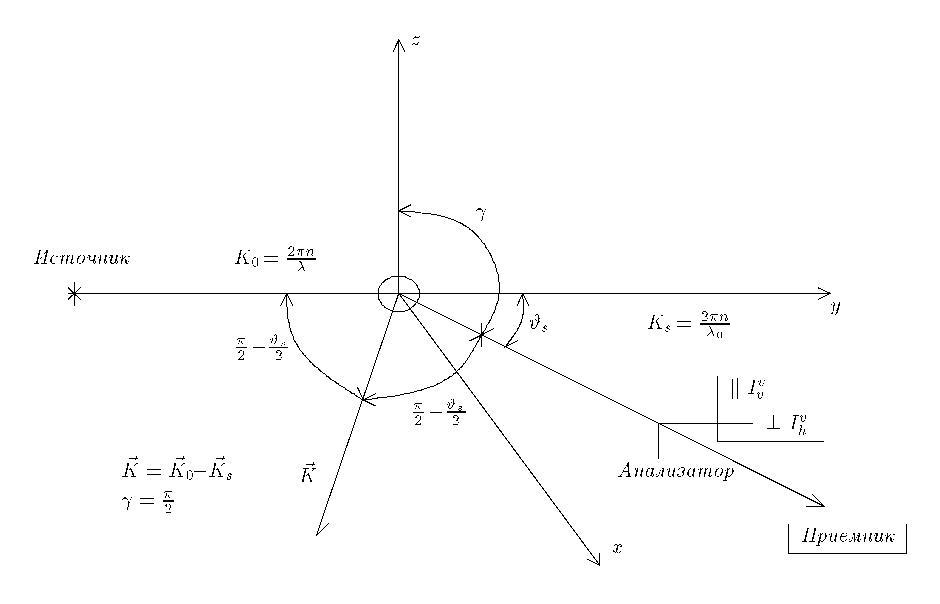
\includegraphics[scale=0.9]{Ris/ris_eps/ris4_4_01.eps}}}

\risp{4.1}{
Основная схема рассеяния}
\par\noindent {\ris Показано плоскополяризованное по оси $z$
($\parallel$) падающее излучение, которое рассеивается по
направлению к приемнику под углами $\gamma$ и $\theta_s$. При
$\gamma={\pi\over2}$ мы выделяем либо поляризованный (вдоль оси
$z$, $\parallel$), либо деполяризованный (в плоскости $xy$,
$\perp$) рассеянный свет, обозначенный $I_v^v$ и $I_h^v$
соответственно. $k_0$ и $k_s$ --- волновые векторы падающего и
рассеянного излучения, $n$ --- показатель преломления
рассеивающей среды, $\lambda_0$ --- длина волны излучения в
вакууме, $\vec K$ --- вектор рассеяния: $\vec K=\vec k_0-\vec
k_s$, $K={4\pi n\over\lambda_0}\left({\theta_s\over2}\right)$.}
\end{figure}

где суммирование по $i$ и по $j$ проводится независимо для $i$-х
членов в момент времени $t=0$ и для $j$-х в момент времени
$t=\tau$. Величина $I_0$ представляет собой интенсивность падающего
плоскополяризованного излучения. Если падающее излучение неполяризовано, то
$$A={\omega_0^4\over c^4R^2}{1\over2}(1+\cos\theta_s)I_0.\noq$$
Формула, определяющая корреляционную функцию $C_y(\tau)$ для
рассеянного света, поляризованного по оси $y$, справедлива для
любого угла $\theta_s$ в плоскости $xy\ (\gamma=\pi/2)$. При ее
получении мы исходим из соотношения
$C_y(\tau)=(c/4\pi)<E_y(t)E_y^*(t+\tau)>$. Столь же справедливо,
однако, и соотношение
$$C_y(\tau)=({c\over4\pi})<E_x(t)E_x^*(t+\tau)>.$$
При рассеянии под углом $\theta_s$ (см. рис. 4.4.1) поле можно
записать в виде линейной комбинации $E_x(t)$ и $E_y(t)$:
$$E_{\theta_s}=E_x\sin\theta_s+E_y\cos\theta_s,$$
где
$$<E_{\theta_s}(t)E_{\theta_s}^*(t+\tau)=\sin^2\theta_s<E_x(t)E_x^*(t+\tau)>
+\cos^2\theta_s<E_y(t)E_y^*(t+\tau)>$$
и $<E_x(t)E_y(t+\tau)>=0$. Теперь легко показать, что
$$<E_x(t)E_x^*(t+\tau)>=<E_y(t)E_y^*(t+\tau)>$$
и, следовательно,
$$<E_{\theta_s}(t)E_{\theta_s}^*(t+\tau)>=<E_x(t)E_x^*(t+\tau)>=
<E_y(t)E_y^*(t+\tau)>.$$
Корреляционные функции, определяемые формулами \eqn{26} и
\eqn{27}, записаны для исходных (при $t=0$) и более поздних (при
$t=\tau$) оложений и ориентаций; угловые скобки обозначают
усреднение по времени или, согласно эргодической гипотезе,
эквивалентное усреднение по ансамблю.

Ориентационная корреляция описывается
членами $\alpha_{zz}^i(0)\alpha_{zz}^j(\tau)$ и
$\alpha_{zy}^i(0)\alpha_{zy}^j(\tau)$, а трансляционная
корреляция --- фазовыми множителями $\exp{-i\vec K\cdot[\vec
r_i(0)-\vec r_j(\tau)]}$. Члены с $i=j$ называют {\it
собственными членами}, с $i\not=j$ --- {\it различными членами}. В
случае газов разумно предположить, что основные вклады будут
давать собственные члены. Разумеется, в жидких кристаллоподобных
системах  (???)  следует ожидать заметных вкладов от членов с
$i\not=j$, а в случае твердых тел эти вклады будут еще больше.

Исследуем теперь природу составляющих тензора поляризуемости,
которые входят в корреляционные функции \eqn{26} и \eqn{27}.
Напомним [см. {\it У. Флайгер}, << Строение и динамика
молекул>>, разд. 6.10],
что при наличии электромагнитного поля с частотой $\omega$
система (молекула) описывается зависящей от времени функцией
$\Psi(\vec r,t)$, выраженной через функции стационарных состояний
$\psi_i(\vec r)$ и коэффициенты $c_i(t)$, зависящие от времени.
Последние определяются выражением для основного взаимодействия,
включающего оператор электрического дипольного момента.
Используя эти результаты, запишем волновую функцию
$k$-го состояния, зависящую от времени, в виде
$$\Psi(\vec r,t)=\psi_k(\vec
r)\exp\left(-{iE_kt\over\hbar}\right)+{\sum\limits_i}'c_i(t)\exp\left(-
{iE_it\over\hbar}\right)\psi_i(\vec r),$$
$$c_i(t)={1\over2\hbar}(\vec E_0\cdot\vec
D)_{ik}\left\{{\exp[i(\omega_{ik}-\omega_0)t]\over
\omega_{ik}-\omega_0}+{\exp[i(\omega_{ik}+\omega_0)t]\over \omega_{ik}+\omega_0}\right\}.\noq$$
Здесь штрих у знака суммы означает, что суммирование не
распространяется на члены с $i=k$; $\omega_0$ --- частота падающего
излучения; $\omega_{ik}=(E_i-E_k)/\hbar$. Из приведенных выше
выражений видно, что система превоначально находилась в $k$-ом
состоянии. Последнее можно представлять себе как
колебательно-вращательное состояние в основном электронном
состоянии, а суммирование по $i$ производится по возбужденным
электронным (колебательно-вращательным) состояниям. Исследуем
теперь для системы, зависящей от времени, матричный элемент
оператора дипольного момента для перехода из состояния $k'$ в
состояние $k$:
$$
(\vec D_{k'k})={\int\psi_{k'}^*(\vec r,t)(\vec D)\psi_k(\vec
r,t)dV\over\int\psi_{k'}^*(\vec r,t)\psi_k(\vec
r,t)dV}=$$ $$
=\int\left[\psi_{k'}^*\exp\left({iE_{k'}t\over\hbar}\right)+{\sum\limits_i}'
c_i^*(t)\exp\left({iE_it\over\hbar}\right)\psi_i^*\right](\vec
D)\times
\times$$ $$
\left[\psi_{k}\exp\left(-{iE_{k}t\over\hbar}\right)+{\sum\limits_i}'
c_i(t)\exp\left(-{iE_it\over\hbar}\right)\psi_i\right]dV=$$ $$
=\vec D_{k'k}\exp(i\omega_{k'k}t)+{\sum\limits_{i}}'\exp(i\omega_{ik}t)c_i^*(t)\vec
D_{ik}+{\sum\limits_{i}}'\exp(i\omega_{k'i}t)c_i(t)\vec
D_{k'i}
$$
где знаменатель равен единице с точностью до членов, ленийных
относительно коэффициентов $c_i(t)$, а меньшие по величине члены
вида $c_i^*(t)c_i(t)$ опущены. Из данного выражения видно, что
$k$ и $k'$ могут соответствовать двум различным
колебательно-вращательным состояниям основного электронного
состояния, а штрихи у знаков суммирования обозначают, что в сумму
не должны входить члены с $i=k$ и $i=k'$ соответственно.
Подставляя, согласно \eqn{29}, коэффициенты $c_i(t)$ в
приведенное выше выражение для $(\vec D)_{k'k}$, получаем
$$
(\vec D)_{k'k}=\exp(i\omega_{k'k}t)\vec D_{k'k}+{\vec
E_0\over2\hbar}\cdot{\sum\limits_i}'\vec D_{ki}\vec
D_{ik'}\times$$ $$
\times \left\{{\exp[i(\omega_{ik}-\omega_{ik'}+\omega_0)t]\over \omega_{ik'}-\omega_0}+
{\exp[i(\omega_{ik}-\omega_{ik'}-\omega_0)t]\over \omega_{ik'}+\omega_0}\right\}+$$ $$
+{\vec E_0\over2\hbar}\cdot{\sum\limits_i}'\vec D_{k'i}\vec
D_{ik}\left\{{\exp[i(\omega_{ik}-\omega_{k'i}+\omega_0)t]\over
\omega_{ik}-\omega_0}+\right.$$ $$
+\left.{\exp[i(\omega_{ik}+\omega_{k'i}+\omega_0)t]\over \omega_{ik}+\omega_0}\right\},$$ $$
\noq$$
где, как отмечено выше, опущены малые члены порядка $|c_i(t)|^2$.
Величина $\vec D_{ki}\vec D_{ik'}$ представляет собой тензор.
Учитывая, что
$$
\omega_{ik}-\omega_{ik'}=\omega_{ik}+\omega_{k'i}= {1\over\hbar}
(E_i-E_k-E_i+E_{k'})=$$ $$
={1\over\hbar}(E_{k'}-E_k)=\omega_{k'k}=-\omega_{kk'},
$$
где $\omega_{ik}$ --- частота электронного перехода, а
$\omega_{kk'}$ --- частота колебательно-вращательного или
вращательного перехода в основном электронном состоянии,
выражение \eqn{30} можно переписать в виде
$$
(\vec D)_{k'k}= \exp(i\omega_{k'k}t)\left\{\vec D_{k'k}+{\vec
E_0\over2\hbar}\cdot{\sum\limits_i}'\vec D_{ki}\vec
D_{ik'}\times\right.$$ $$ 
\times \left[{\exp(i\omega_{0}t)\over \omega_{ik'}-\omega_{0}}+
{\exp(-i\omega_0t)\over \omega_{ik'}+\omega_{0}}\right]+ 
+ \left.{\vec E_0\over2\hbar}\cdot{\sum\limits_i}'\vec D_{k'i}\vec
D_{ik}\left[{\exp(-i\omega_0t)\over \omega_{ik}-\omega_{0}}+
{\exp(i\omega_0t)\over \omega_{ik}+\omega_{0}}\right]\right\}. 
\noq$$
Отметим, что обычно $\omega_{ik}\gg\omega_{k'k}$, поскольку
$\omega_{ik}$ --- угловая частота электронного перехода, а
$\omega_{k'k}$ --- угловая частота колебательного или
вращательного перехода. Таким образом, для случаев
комбинационного и рэлеевского рассеяния разумно предположить, что
$\omega_{ik}\approx\omega_{ik'}$.

При $\omega_{ik}\approx\omega_{ik'}$ выражение \eqn{31} можно
записать в виде
$$\lim\limits_{\omega_{ik}\approx\omega_{ik'}}
(\vec D)_{k'k}= \exp(i\omega_{k'k}t)\left[\vec D_{kk'}+{2\over\hbar}\vec E_0\times\right.$$ 
$${\times \left.{\sum\limits_i}'{\vec D_{ki}\vec
D_{ik'}\omega_{ik}\cos\omega_0t\over(\omega_{ik}^2-\omega_0^2)}\right].\noq$$
Итак, поляризуемость, получаемая из соотношения $\vec D_{\rm
инд}=\vec \alpha\cdot\vec E$, имеет вид
$$\vec\alpha=2\exp(i\omega_{k'k}t){\sum\limits_i}'
{\vec D_{ki}\vec D_{ik'}\omega_{ik}\over\hbar(\omega_{ik}^2-\omega_0^2)}.\noq$$
Общее выражение для тензора поляризуемости \eqn{33} показывает,
что поляризуемость и результирующая интенсивность рассеяния будут
возрастать при $\omega_0\rightarrow\omega_{ik}$. Это условие
резонансного рэлеевского ($k=k'$)  (???)  и резонансного
комбинационного $(k\not=k')$  (???)  рассеяний весьма полезно для
повышения чувствительности рассеяния, если имеется подходящий
источни света с частотой $\omega_0$, близкой к одной из
электронных резонансных частот $\omega_{ik}$. Резонансное
колебательное комбинационное рассеяние оказалось особенно
полезным для идентификации характеристических локальнх колебаний
в определенных местах большой макромолекулы  (???) .

 При помощи направляющих косинусов можно связать тензор
поляризуемости \eqn {33} в неподвижной системе координат $\vec
\alpha(xyz)$ с соответствующим тензором $\vec\alpha(abc)$ в
системе координат, связанной с молекулой. Имеем
$\vec\alpha(xyz)=\vec C\vec\alpha(abc)\tilde{\vec C}$. Согласно
\eqn{26} и \eqn{27}, нам необходимо знать составляющие
$$
\alpha_{zz}= C_{za}\alpha_{aa}C_{az}+C_{zb}\alpha_{bb}C_{bz}+
C_{zc}\alpha_{cc}C_{cz}, 
$$ $$\alpha_{zy}= C_{za}\alpha_{aa}C_{ay}+C_{zb}\alpha_{bb}C_{by}+
C_{zc}\alpha_{cc}C_{cy}. 
\noq$$
Применяя преобразование с учетом направляющих косинусов
в случае аксиально-симметричной молекулы, для которой
$\alpha_{aa}\not=\alpha_{bb}=\alpha_{cc}$ ($a$ --- ось
симметрии), получаем
$$
\alpha_{zz}= \alpha+{2\over3}(\alpha_{aa}-\alpha_{bb})P_2(\cos\theta), 
$$ $$\alpha_{zy}= (\alpha_{aa}-\alpha_{bb})\cos\theta\sin\theta\sin\varphi, \noq$$
где $P_2(\cos\theta)={1\over2}(3\cos^2\theta-1)$ --- полином
Лежандра степени $l=2$ ($a,b$ и $z$ --- оси, лежащие в одной
плоскости, тогда можно сделать преобразование
$\alpha(x,y,z)\rightarrow\alpha(a,b,c)$ через стандартные
сферические полярные углы $\theta$ и $\varphi$). Если
рассеиватель (молекула)
колеблется, необходимо также учесть зависимость составляющих
тензора поляризуемости от колебаний. Это можно сделать путем
разложения каждой составляющей тензора в связанной с молекулой системе
координат по амплитудам молекулярных колебаний, считая их малыми:
$$\alpha_{bb}=\alpha_{aa}^0+\sum\limits_i\left({\partial\alpha_{aa}\over\partial
Q_i}\right)Q_i+\cdots,\noq$$
где $\alpha_{aa}^0$ --- поляризуемость, соответствующая
равновесной конфигурации. Изменение поляризуемости
${\partial\alpha_{aa}\over\partial
Q_i}$, связанное с нормальной координатой $Q_i$, оценивается для
равновесной конфигурации, что обозначено индексом 0.

Таким образом, в настоящем разделе были получены выражения,
необходимые для записи корреляционных функций \eqn{26} и \eqn{27}
в общем случае молекулы, совершающей колебательно-вращательные
движения.

\subzag{Рэлеевское и комбинационное рассеяние в газах,
кинетическая теория и вращательное тушение}

Рассмотрим теперь спектр излучения, рассеянного
аксиально-симметричной молекулой, в предельном случае
разреженного газа, когда средняя длина свободного пробега
рассеивателя (молекулы) велика по сравнению с длинной волны этого
излучения. Начнем с предположения, что вданном предельном случае
разреженного газа в выражения \eqn{26} и \eqn{27} дают вклад лишь
члены с $i=j$. Кроме того, предположим, что для молекулы можно
произвести разделение поступательного, вращательного и
колебательного типов движения. Фазовый множитель поступательного
движения в \eqn{26} и \eqn{27} для молекулы, движущейся со
скоростью $\vec v$, записывается в виде ($i=j$)
$$\exp{-i\vec K\cdot[\vec r_j(0)-\vec r_j(\tau)]}=\exp(i\vec
K\cdot\vec v\tau),\noq$$
где использовано соотношение $\vec r_j(\tau)-\vec r_j(0)=\vec
v\tau$. Применим приближение независимых частиц, подставим
разложение \eqn{36} в формулы \eqn{35}, а затем найденные
результаты подставим, учитывая формулы \eqn{37} и \eqn{33}, в
выражения \eqn{26} и \eqn{27}. Используя эргодическую гипотезу,
получим корреляционные функции для перехода $k\rightarrow k'$
(все перекрестные члены обращаются в нуль в случае изотропного
газообразного образца):
$$
C_z(t)= NA\,\exp(-i\omega_0t)\exp(i\vec K\cdot\vec
vt)P_k\exp(i\omega_{k'k}t)\times 
$$ $$\times \left(\left(\int\psi_{k'}^*\alpha^0\psi_kdV\right)^2+\left\{\int
\psi_{k'}^*\left[{2\over3}(\alpha_{aa}^0-\alpha_{bb}^0)P_2(\cos\theta)\right]\right.\right.\times 
$$ $$\times \left.\
psi_kdV\right\}^2+\left(\int\psi_{k'}^*\left({\partial
\alpha\over\partial Q_j}\right)_0Q_j\psi_kdV\right)^2+ 
$$ $$+ \left.\left\{\int\psi_{k'}^*\left[\left({\partial\alpha_{aa}\over
\partial Q_j}\right)_0-\left({\partial\alpha_{bb}\over\partial
Q_j}\right)_0\right]Q_jP_2(\cos\theta)\psi_kdV\right\}^2\right), 
$$
$$
C_y(t)= NA\,\exp(-i\omega_0t)\exp(i\vec K\cdot\vec
vt)P_k\exp(i\omega_{k'k}t)\times 
$$ $$\times \left(\left[\int
\psi_{k'}^*(\alpha_{aa}^0-\alpha_{bb}^0)\cos\theta\sin\theta\sin\varphi\psi_kdV\right]\right.+ 
$$ $$+ \left.\left\{\int\psi_{k'}^*\left[\left({\partial\alpha_{aa}\over
\partial Q_j}\right)_0-\left({\partial\alpha_{bb}\over\partial
Q_j}\right)_0\right]Q_j\cos\theta\sin\theta\sin\varphi\psi_kdV\right\}^2\right), 
$$ $$P_k= {N_k\over N}.
\noq$$
Здесь N -- полное число рассеивателей, равное $\rho_0V_s$, т. е.
равное числу частиц в единице объема, умноженному на величину
облученного светом объема, сфокусированного на приемник. Величина
$P_k$ представляет собой вероятность того, что система находится
в начальном состоянии $k$, $N_k$ --- число молекул в этом
состоянии. Функция $\psi_k$ является произведением вращательной и
колебательной функции в $k$-ом состоянии, причем усреднение по
электронным волновым функциям учитывается теперь в членах
$\alpha_{aa}^0$, $\alpha_{bb}^0$, $(\partial\alpha_{aa}/\partial Q_j)_0$
и $(\partial\alpha_{bb}/\partial Q_j)_0.$ Матричные элементы
$\psi_{k'}\psi_k$ в выражении для $C_z(t)$, где штрих оозначает
конечное состояние, определяют правила отбора для процессов
рассеяния.

Остановимся теперь подробнее на выражении для $C_z(t)$ в формулах
\eqn{38} и учтем лишь параллельные колебания молекул. Подставляя
функцию $\psi_k=Y_{JM}(\theta,\varphi)\psi_{n_{j}}(Q_j)$, где
$Y_{JM}(\theta,\varphi)$ --- вращательная собственная функция
линейной молекулы и $\psi_{n_{j}}(Q_j)$ --- функция
гармонического осциллятора для $j$-й параллельной моды ($n_j$
характеризует колебательное состояние), получаем следующее
выражение для $C_z(t)$:
$$
C_z(t)= A\,\exp(-i\omega_0t)\exp(i\vec K\cdot\vec
vt)\left(N(\alpha^0)^2+N_{JM}\exp(i\omega_Rt)\times\right. 
$$ $$\times \left[{4\over3}\left({\pi\over5}\right)^{1/2}(\alpha_{aa}^0-\alpha_{bb}^0)
\int\limits_0^{2\pi}\int\limits_0^{\pi}Y^*_{JM}Y_{20}Y_{J'M'}\sin\theta
d\theta d\varphi\right]^2+ 
$$ $$+ N_{n_{j}}\exp(i\omega_jt)\left[\left({\partial\alpha\over\partial
Q_j}\right)_0<n_j|\theta_j|n'_j>\right]^2+ 
$$ $$+ N_{n_{j}JM}\exp(i\omega_{jR}t)\left\{{4\over3}\left({\pi\over5}\right)^{1/2}
\left[{\partial(\alpha_{aa}-\alpha_{bb})\over\partial
Q_j}\right]_0<n_j|Q_j|n'_j>\right.\times 
$$ $$\times \left.\left.\int\limits_0^{2\pi}\int\limits_0^{\pi}Y^*_{JM}Y_{20}Y_{J'M'}\sin\theta
d\theta d\varphi\right\}\right), 
$$ $$\omega_R= {(E_{J'M'}-E_{JM})\over\hbar},\hskip
4mm\omega_j={(E_{n'_{j}}-E_{n_{j}})\over\hbar}, 
$$ $$\omega_{jR}= {(E_{n'_{j}}+E_{J'M'}-E_{n_{j}}-E_{JM})\over\hbar}, 
\noq$$
где также использована функция
$P_2(\cos\theta)=2(\pi/5)^{1/2}Y_{20}$. В формуле \eqn{39}
$\omega_R$ --- чисто вращательная частота, $\omega_j$ --- чисто
колебательная частота, а $\omega_{jR}$ ---
колебательно-вращательная частота. $N$ --- полное число
рассеивателей; $N_{JM}$ --- число молекул, находящихся во
вращательном состоянии $JM$; $N_{n_{j}}$ --- число молекул,
находящихся в $n$-м состоянии $j$-й колебательной моды;
$N_{n_{j}JM}$ --- число молекул, находящихся в
колебательно-вращательном состоянии $n_j,\ JM$. Первый член в
формуле \eqn{39} соответствует рэлеевскому рассеянию с весовым
множителем $(\alpha^0)^2$. Второй член описывает чисто
вращательное комбинационное рассеяние с правилами отбора $\Delta
J=0,\ \pm2,\ \Delta M=0$; для амплитудного множителя, зависящего
от вращения, мы введем обозначение
$$f_{JM}=N_{JM}\left[{4\over3}\left({\pi\over5}\right)^{1/2}
(\alpha_{aa}^0-\alpha_{bb}^0)\int\limits_0^{2\pi}\int\limits_0^{\pi}
Y^*_{JM}Y_{20}Y_{J'M'}\sin\theta
d\theta d\varphi\right]^2.\noq$$
Третий член соответствует чисто колебательному комбинационному
рассеянию с правилами отбора $\Delta n=+1$ для гармонического
осциллятора; амплитуду колебательного рассеяния для $j$-й
параллельной моды мы обозначим как
$$f_j=N_{n_{j}}\left[\left({\partial\alpha\over\partial
Q_j}\right)_0<n_j|Q_j|n'_j>\right]^2.\noq$$
Четвертый член в формуле \eqn{39} описывает
колебательно-вращательное комбинационное рассеяние с правилами
отбора $\Delta n=+1,\ \Delta J=0,\ \pm2,\ \Delta M=0$, и для
амплитуды колебательно-вращательного рассеяния мы применим
обозначение
$$
f_{JM_j}= N_{n_{j}JM}\left\{{4\over3}\left({\pi\over5}\right)^{1/2}
\left[\left({\partial\alpha_{aa}\over\partial
Q_j}\right)_0-\left({\partial\alpha_{bb}\over\partial
Q_j}\right)_0\right]<n_j|Q_j|n'_j>\times\right. 
$$ $$\times \left.\int\limits_0^{2\pi}\int\limits_0^{\pi}
Y^*_{JM}Y_{20}Y_{J'M'}\sin\theta
d\theta d\varphi\right\}^2. 
\noq$$
подставляя выражения \eqn{40}, \eqn{41} и \eqn{42} в \eqn{39},
получаем
$$
C_z(t)= A\,\exp(-i\omega_0t)\exp(i\vec K\cdot\vec
vt)[N(\alpha^0)^2+ 
$$ $$+ f_{JM}\exp(i\omega_Rt)+f_j\exp(i\omega_jt)+f_{JM_{j}}\exp(i\omega_{jR}t)]. 
\noq$$
Отметим здесь, что формула \eqn{43} была выведена для случая лишь
одной скорости молекул $\vec v$ в приближении независимых частиц
при отсутствии столкновительной релаксации. Теперь мы учтем
усредненное по Больцману распределение скоростей, а также
процессы релаксации, как вращательной, так и колебательной.

Рассмотрим сначала усреднение по скорости фазового множителя
$\exp(i\vec K\cdot\vec vt)$ в выражении \eqn{43}. Усреднение
множителя $\exp(i\vec K\cdot\vec vt)$ по всем скоростям в
трехмерном пространстве проводится путем обобщения нормированной
функции распределения Максвелла-Больцмана с учетом вероятности
различных значений скоростей:
$$
[\exp(i\vec K\cdot\vec vt)_{\rm ср}= \left({M\over2\pi
kT}\right)^{3/2}\int\limits_{-\infty}^{\infty}\int\limits_{-\infty}^{\infty}
\int\limits_{-\infty}^{\infty}\exp(i\vec K\cdot\vec vt)\times 
$$ $$\times \exp\left[-{M\over2kT}(v_x^2+v_y^2+v_z^2)\right]dv_xdv_ydv_z= 
$$ $$= \exp\left[-\left({kt\over2M}\right)K^2t^2\right]. 
\noq$$
Полуширина этой гауссовой кривой (в шкале времени) равна
$$\Delta t={1\over K}\left({2M\ln2\over kT}\right)^{1/2}.\noq$$

Учтем, наконец, эффекты первого порядка релаксации молекул во
вращательном $(\tau_R)$ и колебательном $(\tau_V)$ состояниях,
причем следует ожидать, что $\tau_V\gg\tau_R$. Вводя
соответствующие релаксации первого порядка в выражение \eqn{43} и
подставляя соотношение \eqn{44} для усреднения по скоростям,
получаем
$$
C_z(t)= A\,\exp(-i\omega_0t)\exp\left[
-\left({kT\over2M}\right)K^2t^2\right]\left[
N(\alpha^0)^2+\right. 
$$ $$+ f_{JM}\exp(i\omega_Rt)\exp\left(-{t\over\tau_R}\right)+
f_j\exp(i\omega_jt)\exp\left(-{t\over\tau_j}\right)+ 
$$ $$+ \left.f_{JM_{j}}\exp(i\omega_{jR}t)\exp\left(-{t\over\tau_R}\right)\exp
\left(-{t\over\tau_j}\right)\right]. 
\noq$$
Здесь $N$ --- число рассеивателей, $A$ определено выражениями
\eqn{27} и \eqn{28}, $f_{JM},\ f_j$ и $f_{JM_j}$ определены
формулами \eqn{40}, \eqn{41} и \eqn{42} соответственно, $\tau_R$
--- время вращательной релаксации вращательного состояния $JM$, а
$\tau_j$ --- время колебательной релаксации $j$-го колебательного
состояния.

Для выражения \eqn{46} имеются два интересных предельных случая:
случай низких давлений, когда члены затухания
$\exp[-(kT/2M)K^2t^2]$ доминируют по сравнению с релаксационными
членами $\exp(-t/\tau_R)$ и $\exp(-t/\tau_j)$, и случай очень
высоких давлений, когда релаксационные члены превышают гауссов
член затухания $\exp[-(kT/2M)K^2t^2]$. Рассмотрим теперь спектры,
получающиеся в этих двух предельных случаях. Подставляя выражение
\eqn{46} в формулу \eqn{22} получаем интенсивность, расчитанную
на единичный интервал частот, для $N$ рассеивателей {величина
$\Delta t$ определена согласно \eqn{45}.

\noindent{\it Низкое давление:} $\Delta t\ll\tau_R,\ \Delta
t\ll\tau_j$
$$
I_v^v(\omega)= {1\over\pi}\hbox{Re}\int\limits_0^{\infty}C_z(t)\exp(i\omega
t)dt= 
$$ $$= {A\over K}\left({M\over2\pi
kT}\right)^{1/2}\left\{N(\alpha^0)^2\exp\left[-\left({M\over2K^2k
T}\right)(\omega-\omega_0)^2\right]+\right. 
$$ $$+ f_{JM}\exp\left[-\left({M\over2K^2k
T}\right)(\omega+\omega_R-\omega_0)^2\right]+ 
$$ $$+ f_{j}\exp\left[-\left({M\over2K^2k
T}\right)(\omega+\omega_j-\omega_0)^2\right]+ 
$$ $$+ \left.f_{JM_j}\exp\left[-\left({M\over2K^2k
T}\right)(\omega+\omega_{jR}-\omega_0)^2\right]\right\}.
\noq$$
{\it Высокое давление}: $\Delta t\gg\tau_R,\ \Delta t\gg\tau_j$
$$
I_v^v(\omega)= {NA\over K}\left({M\over2\pi k
T}\right)^{1/2}(\alpha^0)^2\exp\left[-\left({M\over2K^2kT}\right)
(\omega-\omega_0)^2\right]+ 
$$ $$+ {A\over\pi}f_{JM}\left[{(1/\tau_R)\over(1/\tau_R)^2+(\omega+\omega_R-\omega_0)^2}\right]+ 
$$ $$+ {A\over2\pi}f_{j}\left[{(1/\tau_j)\over(1/\tau_j)^2+(\omega+\omega_j-\omega_0)^2}\right]+ 
$$ $$+ {A\over2\pi}f_{JM_j}\left[{(1/\tau_j+1/\tau_R)\over(1/\tau_j+1/\tau_R)^2+(\omega+\omega_{jR}-\omega_0)^2}\right]. 
\noq$$
Первые члены в формулах \eqn{47} и \eqn{48} соответствуют
рэлеевскому рассеянию, вторые члены с частотами вокруг
$(\omega_0-\omega_R)$ --- чисто вращательному комбинационному
рассеянию, третьи члены с частотами вокруг $(\omega_0-\omega_j)$
--- чисто колебательному комбинационному рассеянию, а четвертые
члены с частотами вокруг $(\omega_0-\omega_{jR})$ ---
колебательно-вращательному комбинационному рассеянию [определения
$\omega_R,\ \omega_j,\ \hbox{и}\ \omega_{jR}$ см. в \eqn{39}].
Все четыре члена в выражении \eqn{47} при доплеровском уширении в
предельном случае низких давлений представляют собой гауссовы
кривые с полуширинами $\Delta\omega=K(2kT\ln2/M)^{1/2}$, где $K$
--- величина вектора рассеяния. Таким образом, нами получен
весьма интересный результат: полуширина пропорциональна вектору
рассеяния $K=(4\pi/\lambda)\sin(\theta_s/2)$. Отсюда вытекает,
что в данном предельном случае низких давлений при малых углах
рассеяния может быть достигнуто очень высокое разрешение (см.
рис. 4.4.1). Экспериментальную проверку этого вывода можно найти
в работе  (???) .

В предельном случае высоких давлений формула \eqn{48} приводит к
гауссовому контуру линий для рэлеевского рассеяния (с центром в
точке $\omega_0$) и к лоренцевой форме для всех типов
комбинационного рассеяния. Полуширины для остающихся членов равны
$\Delta\omega={1\over\tau_R}$ для чисто вращательного члена,
$\Delta\omega={1/\tau_j}$ для чисто колебательного члена и
$\Delta\omega=(1/\tau_j+1/\tau_R)$ для колебательно-вращательного
члена.

В промежуточном случае, когда существенны как эффект Доплера, так
и процессы релаксации, непосредственное фурье-преобразование
выражения \eqn{46} позволяет получить спектр. Последний будет
представлять собой свертку гауссовых и лоренцевых
кривых\footnote{*}{Подробности см. {\it У. Флайгер}, Динамика и
свойства молекул, разд. 7.2}.

Отметим также, что, согласно определению коэффициентов $f$ в
\eqn{40}, \eqn{41} и \eqn{42} и множителя $N_k$ в \eqn{38}, при
$E(n_jJM)>E(n'_jJ'M')$ и любой комбинации квантовых чисел $n_j,\
J,\ M,\ n'_j,\ J'$ и $M'$ (штрихи отвечают конечному состоянию)
величина $\omega_{n'_jJ'M'}$ является отрицательной. Это приводит
к возрастанию частот комбинационного рассеяния по сравнению с
частотой пдающего излучения $\omega_0$. Такие переходы называют
{\it антистоксовыми переходами. Стоксовы переходы} приводят к
появлению частот, меньших чем $\omega_0$, благодаря условию
$E(n_jJM)<E(n'_jJ'M')$, приводящему к положительным значениям
величины $\omega_{n'_jJ'M',n_jJM}$. Разумеется, из определения
множителя $N_k$ согласно \eqn{38} следует также, что стоксовы
переходы $[E(n_jJM)<E(n'_jJ'M')]$ будут более интенсивны, чем
антистоксовы $[E(n_jJM)>E(n'_jJ'M')]$.

Вернемся теперь к выражению \eqn{38} для $C_y(t)$. Подставляя
соотношение
$$\cos\theta\sin\theta\sin\varphi=i\left({2\pi\over15}\right)^{1/2}(Y_{2-1}-Y_{21})$$
и проделывая все преобразования, описаные вслед  \eqn{38},
получаем для $C_y(t)$ выражение, аналогичное \eqn{46}:
$$
C_y(t)= A\exp(-i\omega_0t)\exp\left[-\left({kT\over
M}\right)K^2t^2\right]\times 
$$ $$\times \left[f'_{JM}\exp(-i\omega_Rt)\exp\left(-{t\over\tau_R}\right)+\right. 
$$ $$+ \left.f'_{JM_j}\exp(-i\omega_{jR}t)\exp\left(-{t\over\tau_R}\right)\exp\left(-{t\over\tau_j}\right)\right], 
$$
$$
f'_{JM}=N_{JM}\left({2\pi\over15}\right)
\left[(\alpha^0_{aa}-\alpha_{bb}^0)\int\limits_0^{2\pi}\int\limits_0^{2\pi}
Y^*_{JM}(Y_{2-1}\right. -Y_{21})\times 
$$ $$\times \left.Y_{J'M'}\sin\theta d\theta d\varphi\right]^2, 
$$
$$
f'_{JM_j}=N_{n_jJM} \left({2\pi\over15}\right)\left\{\left[\left({\partial
\alpha_{aa}\over\partial
Q_j}\right)_0-\left({\partial\alpha_{bb}\over\partial
Q_j}\right)_0\right]<n'_j|Q_j|n_j>\times\right. 
$$ $$\times \left.\int\limits_0^{2\pi}\int\limits_0^{2\pi}
Y^*_{JM}(Y_{2-1}-Y_{21})Y_{J'M'}\sin\theta d\theta
d\varphi\right\}^2.
\noq$$
Таким образом, корреляционная функция $C_y(t)$, приводящая к
деполяризованным спектрам, включает в себя чисто вращательный
член с правилами отбора $\Delta J=0,\ \pm2,\ \Delta M=\pm1$ и
колебательно-вращательный член с правилами отбора для
параллельных колебаний $\Delta n_j=\pm1,\ \Delta J=0,\ \pm2,
\Delta M=\pm 1$. Частотно-временн$\acute{\hbox{о}}$е
фурье-преобразование функции $C_y(t)$ \eqn{49} для получения
спектральной функции $I_h^v(\omega)$ производится по методике,
описанной ранее при получении функции $I_v^v(\omega)$ в обоих
предельных случаях высоких и низких давлений. Непосредственное
выполнение этих преобразований предоставляется читателю.
Дополнительные подробности, касающиеся динамики молекул и
рассеяния света в газах, можно найти  (???) .

Вернемся теперь к выражениям \eqn{26} и \eqn{27} и исследуем
корреляционные функции для случая очень высоких давлений или
конденсированной фазы (жидкости), когда время между
столкновениями мало по сравнению с периодом вращения молекулы. В
этом предельном случае вращательного тушения понятие
вращательного состояния теряет смысл, и для вывода корреляционных
функций, позволяющих получить спектры, необходимо использовать
иной подход. Для простоты рассмотрения предположим сначала, что
молекула представляет собой жесткий неколеблющийся волчок.
Подставляя формулы \eqn{35} в \eqn{26} и \eqn{27}, получаем
$$\parallel\hskip 7 true mm
C_z(t)={c\over4\pi}<E_z(0)E_z^*(t)>=A\left<\sum\limits_{i,j}\left[\alpha+{2\over3}
(\alpha_{aa}-\alpha_{bb})P_2(\cos\theta)\right]_{0i}\times\right.$$$$\times\left[\alpha+{2\over3}
(\alpha_{aa}-\alpha_{bb})P_2(\cos\theta)\right]_j\times\exp(-i\omega_0t)\exp\{i\vec
K[\vec r_i(0)-\vec r_j(t)]\}\Bigg>,\noq$$
$$\perp\hskip 7 true mm
C_y(t)={c\over4\pi}<E_y(0)E_y^*(t)>=A\left<
\sum\limits_{i,j}(\cos\theta\sin\theta\sin\varphi)_{0i}\times\right.$$$$\times(\cos\theta\sin\theta
\sin\varphi)_j(\alpha_{aa}-\alpha_{bb})_{0i}\times
(\alpha_{aa}-\alpha_{bb})_j\exp(-i\omega_0t)\exp\left\{-i\vec K[\vec
r_i(0)-\vec r_j(t)]\right\}\Bigg>,\noq$$
где из-за вращения молекулы $\theta$ и $\varphi$ зависят от времени.
Индекс 0 указывает, что значения величин в
корреляционных функциях взяты при $t=0$. Если рассеиватели
ориентированы в пространстве хаотически (изотропное
распределение), то средние значения перекрестных членов $\alpha
P_2(\cos\theta)_i$ и $\alpha P_2(\cos\theta)_j$ в \eqn{50}
обращаются в нуль. Предположим также, что все неколеблющиеся
молекулы или рассеиватели в газе, жидкости и твердом теле эквивалентны, а величины
$\alpha$ и $(\alpha_{aa}-\alpha_{bb})$ не зависят от времени.
Тогда можно переписать выражения \eqn{50} и \eqn{51} следующим образом:
$$C_z(t)=A\exp(-i\omega_0t)\alpha^2\left<\sum\limits_{i,j}\exp\left\{
-i\vec K[\vec r_i(0)-\vec r_j(t)]\right\}\right>+$$$$+{4\over9}A
\exp(-i\omega_ot)(\alpha_{aa}-\alpha_{bb})^2\left<\sum\limits_{i,j}P_2(\cos\theta)_{0i}P_2(\cos\theta)_j\times
\exp\left\{-i\vec K[\vec r_i(0)-\vec r_j(t)]\right\}\right>,\noq$$
$$C_y(t)=A\exp(-i\omega_0t)(\alpha_{aa}-\alpha_{bb})^2\times$$$$\times\left<\sum\limits_{i,j}
(\cos\theta\sin\theta\sin\varphi)_{0i}\times(\cos\theta\sin\theta\sin\varphi)_j
\times\exp\left\{-i\vec K[\vec r_i(0)-\vec
r_j(t)]\right\}\right>.\noq$$
Как было отмечено при обсуждении, следующем за формулой \eqn{28},
члены с $i=j$ называют {\it собственными членами}, а члены с
$i\not=j$ --- {\it различными членами}.
Hа основании эргодической гипотезы корреляционные функции для
одинаковых рассеивателей записываются с учетом усреднения по всем
положениям и ориентациям в виде
$$C_z(t)=A\exp(-i\omega_0t)N\alpha^2\int\limits_{V_s}\exp(i\vec
K\cdot\vec R)P(\vec
R,t)dV_s+{4\over9}A\exp(-i\omega_0t){N(\alpha_{aa}-\alpha_{bb})\over4\pi}\times$$
$$\times\int\limits_{0}^{2\pi}
\int\limits_{0}^{2\pi}\int\limits_{-1}^{1}\int\limits_{-1}^{1}\int\limits_{V_s}
\exp(i\vec K\cdot\vec R)\times P_2(\cos\theta_0)P_2(\cos\theta)P(\vec
R,\theta,\varphi,t)dV_sd\cos\theta_0d\cos\theta
d\varphi_0d\varphi,\noq$$
$$C_y(t)=A\exp(-i\omega_0t){N(\alpha_{aa}-\alpha_{bb})\over4\pi}\int\limits_{0}^{2\pi}
\int\limits_{0}^{2\pi}\int\limits_{-1}^{1}\int\limits_{-1}^{1}\int\limits_{V_s}
\exp(i\vec K\cdot\vec
R)\times$$$$\times(\cos\theta\sin\theta\sin\varphi)_0(\cos\theta\sin\theta\sin\varphi)
\times P(\vec R,\theta,\varphi,t)dV_sd\cos\theta_0\cos\theta
d\varphi_0d\varphi,\noq$$
где для удобства интеграл $\int\limits_0^{\pi}\sin\theta d\theta$
заменен интегралом $\int\limits_{-1}^1d\cos\theta$.
Величина $N$ представляет собой число рассеивателей в
рассеивающем объеме $V_s$, $dV_s$ ---
элемент объема, и соответствующий интеграл охватывает рассеивающий
объем (облучаемый объем, сфокусированный на приемник). В
записанных выражениях
функции $P(a)$ представляют собой
пространственно-временн$\acute{\hbox{ы}}$е и
ориентационно-пространственно-временн$\acute{\hbox{ы}}$е корреляционные
функции.
$P(\vec R,t)$ --- рассчитанная на единицу объема
вероятность того, что если в момент времени $t=0$ центр рассеяния
находится в точке $\vec R=0$, то в момент $t$ будет иметься центр
рассеяния в точке $\vec R$. Таким образом, очевидно, что $P(\vec
R,t)$ содержит пространственные и временн$\acute{\hbox{ы}}$е члены,
как собственные, так и различные.
$P(\vec R,\theta,\varphi,t)$ представляет собой
ориентационно-пространственно-временн$\acute{\hbox{у}}$ю
корреляционную функцию.
Она дает рассчитанную на единицу объема вероятность того, что если
центр взаимодействия частицы с ориентацией $\theta_0$ и $\varphi_0$
находился в точке $\vec R=0$ в момент времени $t=0$, то будет
иметься также частица с ориентацией $\theta$ и $\varphi$ в точке $\vec R$ в
момент времени $t$. Дополнительный множитель ${1\over4\pi}$, связанный с
вероятностями $P(\vec R,\theta,\varphi,t)$, получается в
предположении нормировки вероятностей при начальных условиях в момент
$t=0$. Если $P(\vec R,t)=\delta(\vec R)$, т. е.
трехмерной дельта функции при $t=0$, то имеем
$$\int\limits_{V_s}\exp(i\vec K\cdot\vec R)P(\vec
R,0)dV_s=\int\limits_{V_s}\exp(i\vec K\vec R)\delta(\vec
R)dV_s=1,\noq$$
а если $P(\vec R,\theta,\varphi,t)=\delta(\vec
R)\delta(\cos\theta-\cos\theta_0)\times\delta(\varphi-\varphi_0)$,
то имеем
$$\int\limits_{0}^{2\pi}\int\limits_{0}^{2\pi}\int\limits_{-1}^{1}\int
\limits_{-1}^{1}\int\limits_{V_s}\exp(i\vec K\cdot\vec R)P(\vec
R,\theta,\varphi,t)dV_sd\cos\theta_0d\cos\theta
d\varphi_0d\varphi=$$
$$=\int\limits_{0}^{2\pi}\int\limits_{0}^{2\pi}\int\limits_{-1}^{1}\int
\limits_{-1}^{1}\int\limits_{V_s}\exp(i\vec K\cdot\vec
R)\delta(\vec
R)\delta(\cos\theta-\cos\theta_0)\times\delta(\varphi-\varphi_0)dV_s
d\cos\theta_0 d\cos\theta
d\varphi_0d\varphi=$$$$=\int\limits_{0}^{2\pi}
\int\limits_{-1}^{1}d\cos\theta_{0}d\varphi_0=4\pi.\noq$$
В результатах \eqn{56} и \eqn{57} использовано важное приближение, согласно
которому предполагается, что интеграл по рассеивающему объему
$V_s$ сохраняет смысл при $R\rightarrow\infty$. Это приближение
является достаточно хорошим, если размеры рассеивателя малы по
сравнению с фактическим рассеивающим объемом.
Использование данного приближения приводит к преобразованию Фурье трехмерной
дельта-функции $\delta(\vec R)$ в формулах \eqn{56} и \eqn{57},
дающему единицу. В более общем случае можно записать
$$\int\limits_{V_s}\exp(i\vec K\cdot\vec R)\cdot P(\vec
R,t)dV_s\approx \overline{P}(K,t).\noq$$
Таким образом $\overline{P}(K,t)$ --- трехмерный пространственный фурье-образ
$P(\vec R,t)$.

Выражения \eqn{54} и \eqn{55} будут широко использоваться далее
для описания рассеяния системами с вращательным тушением.
Для получения выражений для $P(\vec R,t)$ и
$P(\vec R,\theta,\varphi,t)$ мы воспользуемся гидродинамическими
теориями. Так, например, выражение для $P(\vec R,t)$ в первом
члене формулы \eqn{54} получается в случае чистой жидкости путем
решения трех связанных уравнений --- уравнения непрерывности,
уравнения Навье --- Стокса и уравнения переноса энергии, что
приводит к рассеянию Рэлея --- Бриллюэна.


Полные интенсивности получаются из выражений для $C_z\ (t=0)$ и
$C_y\ (t=0)$ путем подстановки соответствующих начальных или
статических условий в \eqn{54} и \eqn{55}. Используя $P(\vec
R,0)$ и $P(\vec R,\theta,\varphi,0)=P(\vec
R,0)\delta(\cos\theta-\cos\theta_0)\delta(\varphi-\varphi_0)$
в \eqn{54} и \eqn{55}, а также формулу (II.14), находим
интенсивности
$$I_v^v=C_z(0)=AN\overline{P}
(K,0)\left[\alpha^2+{4\over45}(\alpha_{aa}-\alpha_{bb})^2\right],\noq$$
$$I_h^v=C_y(0)=AN\overline{P}
(K,0){1\over15}(\alpha_{aa}-\alpha_{bb})^2.\noq$$
Таким образом, если падающее излучение поляризовано вдоль оси
$z$, а наблюдение ведется в плоскости $xy$, отношение
интенсивностей перпендикулярно и параллельно поляризованного
света равно
$$\Delta={I_h^v\over I_v^v}={C_y(0)\over
C_z(0)}={{1\over15}(\alpha_{aa}-\alpha_{bb})^2\over\alpha^2+{4\over45}(\alpha_{aa}
-\alpha_{bb})^2}={3(\alpha_{aa}-\alpha_{bb})^2\over45\alpha^2+4(\alpha_{aa}-\alpha_{bb})^2}.\noq$$
Таким образом, имеем хорошо известное выражение для степени
деполяризации. Вильсон, Дешиус и Кросс  (???) , используя
аналогичные методы, получили ряд выражений для степени
деполяризации. Выражения \eqn{59} и \eqn{60} обобщаются на случай
молекул любого типа путем замены
$(\alpha_{aa}-\alpha_{bb})^2$ на
$$\gamma^2={1\over2}\left\{(\alpha_{aa}-\alpha_{bb})^2+(\alpha_{bb}-\alpha_{cc})^2
+(\alpha_{cc}-\alpha_{aa})^2\right\}.$$
Возвращаясь теперь к формулам \eqn{59} и \eqn{60}, запишем
$$I_{v}^v=I_{\rm из}+{4\over3}I_{\rm аниз},\hskip 4mm
I_h^v=I_v^h=I_h^h=I_{\rm аниз}.\noq$$
Обозначения $I_v^v$ и $I_h^v$ проиллюстрированы на рис. 4.4.1;
другие типы обозначений $I_{\rm набл}^{\rm пад}$ также
понятны из геометрической схемы опыта, изображенной на рисунке.
Выражение для $I_h^h$ легко выводится, причем соответствующая
корреляционная функция совпадает с \eqn{53} или \eqn{55} с
заменой произведения $\cos\theta\sin\theta\sin\varphi$ на
$\sin^2\theta\sin\varphi\cos\varphi$. При этом легко показать,
что имеет место соотношение \eqn{61} $I_h^h=I_h^v$.

Если падающее излучение неполяризовано, отношение интенсивностей
перпендикулярно и параллельно поляризованного рассеянного света
определяется формулой $(I_b^a=I_{\rm набл}^{\rm пад})$
$${I_h^{\rm неполяриз}\over
I_v^{\rm неполяриз}}={I_h^v+I_{h}^h\over
I_v^v+I_v^h}={2I_h^v\over
I_v^v+I_v^h}={6(\alpha_{aa}-\alpha_{bb})^2\over45\alpha^2+7(\alpha_{aa}-\alpha_{bb})^2}.\noq$$

Вернемся теперь к формулам \eqn{26} и \eqn{27} и повторим
описанный путь от формул \eqn{50} и \eqn{51} до формул \eqn{54} и
\eqn{55}, включая учет параллельных колебаний линейной молекулы.
Подставляя выражения \eqn{35} и \eqn{36} в \eqn{26} и \eqn{27} и
повторяя приведенный выше анализ тушения вращательных состояний
[а также используя \eqn{58}], получаем
$$
C_z(t)= A\,\exp(-i\omega_0t)N(\alpha^0)^2\overline{P}
(K,t)+{4A\over9}\exp(-i\omega_0t)\times 
$$ $$\times {N(\alpha^0_{aa}-\alpha_{bb}^0)^2\over4\pi}\overline{P}
(K,\theta,\varphi,t)+ 
$$ $$+ A\exp(-i\omega_0t)\exp(i\omega_{n'_j,n_j}t)\overline{G}
(K,t)f_j\exp\left(-{t\over\tau_j}\right)+ 
$$ $$+{4A\over9}\exp (-i\omega_0t)\exp(i\omega_{n'_j,n_j}t)\left({N\over4\pi}\right)
\overline{G}(K,\theta,\varphi,t)h_j\exp\left(-{t\over\tau_j}\right), 
$$ $$C_y(t)= A\,\exp(-i\omega_0t){N(\alpha_{aa}^0-\alpha_{bb}^0)^2\over4\pi}\overline{\overline{P}}
(K,\theta,\varphi,t)+ 
$$ $$+A\,\exp (-i\omega_0t)\exp(i\omega_{n'_j,n_j}t)\left({N\over4\pi}\right)
\overline{\overline{G}}(K,\theta,\varphi,t)h_j\exp\left(-{t\over\tau_j}\right), 
$$
$$
\overline{P}(K,t)= \int\limits_{V_s}\exp(i\vec K\cdot\vec
R)P(\vec R,t)dV_s 
\overline{P}(K,\theta,\varphi,t)= $$ $$ =\int\limits_{0}^{2\pi}\int\limits_{0}^{2\pi}
\int\limits_{-1}^{1}\int\limits_{-1}^{1}\int\limits_{V_s}\exp(i\vec
K\cdot\vec R)P_2(\cos\theta_0)P_2(\cos\theta)\times 
$$ $$\times P(\vec R,\theta,\varphi,t)dV_sd\cos\theta_0d\cos\theta
d\varphi_0d\varphi, 
$$ $$\overline{G}(K,t)= \int\limits_{V_s}\exp(i\vec K\cdot\vec
R)G(\vec R,t)dV_s, 
$$ $$\overline{G}(K,\theta,\varphi,t)= \int\limits_{0}^{2\pi}\int\limits_{0}^{2\pi}
\int\limits_{-1}^{1}\int\limits_{-1}^{1}\int\limits_{V_s}\exp(i\vec
K\cdot\vec R)P_2(\cos\theta_0)P_2(\cos\theta)\times 
$$ $$\times G(\vec R,\theta,\varphi,t)dV_sd\cos\theta_0d\cos\theta
d\varphi_0d\varphi, 
$$ $$\overline{\overline{P}}(K,\theta,\varphi,t)= \int\limits_{0}^{2\pi}\int\limits_{0}^{2\pi}
\int\limits_{-1}^{1}\int\limits_{-1}^{1}\int\limits_{V_s}\exp(i\vec
K\cdot\vec R)(\cos\theta\sin\theta\sin\varphi)_0\times 
$$ $$\times (\cos\theta\sin\theta\sin\varphi)P(\vec
R,\theta,\varphi,t)dV_sd\cos\theta_0d\cos\theta
d\varphi_0d\varphi, 
$$ $$\overline{\overline{G}}(K,\theta,\varphi,t)= \int\limits_{0}^{2\pi}\int\limits_{0}^{2\pi}
\int\limits_{-1}^{1}\int\limits_{-1}^{1}\int\limits_{V_s}\exp(i\vec
K\cdot\vec R)(\cos\theta\sin\theta\sin\varphi)_0\times 
$$ $$\times (\cos\theta\sin\theta\sin\varphi)G(\vec
R,\theta,\varphi,t)dV_sd\cos\theta_0d\cos\theta
d\varphi_0d\varphi, 
$$ $$f_j= {1\over2}N_{n_j}\left[\left({\partial\alpha\over\partial
Q_j}\right)_0<n_j|Q_j|n'_j>\right]^2, 
$$ $$h_j= {1\over2}N_{n_j}\left[\left({\partial(\alpha_{aa}-\alpha_{bb})\over\partial
Q_j}\right)_0<n_j|Q_j|n'_j>\right]^2, 
$$ $$\omega_{n'_j,n_j}= {E_{n'_j}-E_{n_j}\over\hbar}. 
\noq$$
Здесь $N_{n_j}$ --- число молекул в состоянии $n_j$. Первые два
члена в выражении для $C_z(t)$ совпадают с результатом \eqn{54},
а первый член в выражении для $C_y(t)$ --- с результатом
\eqn{55}. Остальные члены в этих выражениях обязаны наличию
параллельных колебаний аксиально-симметричной молекулы
$(\alpha_{aa}\not=\alpha_{bb}=\alpha_{cc})$. Вероятностные
функции $P(\vec R,t)$ и $P(\vec R,\theta,\varphi,t)$ и их
пространственные фурье-образы (включающие усреднение по
ориентациям) обсуждались ранее. Они содержат как собственные, так
и различные члены. Функции $G(\vec R,t)$ и $G(\vec
R,\theta,\varphi,t)$ отличаются от функций
$P(\vec R,t)$ и $P(\vec R,\theta,\varphi,t)$ тем, что содержат
лишь собственные члены. Это связано с тем, что различные члены в
функциях $G$ соответствуют колебаниям пар различных молекул,
имеющим призвольные фазы относительно друг друга. Таким образом,
следует ожидать, что различные члены, включающие суммирование по
парам колеблющихся молекул, обратятся в нуль. Разумеется, если
исследуется система, в которой различными членами вообще можно
пренебречь, функции $G$ и $P$ идентичны. В корреляционных
функциях \eqn{64} учтены также экспоненциальные процессы
колебательной релаксации, для которых $\tau_j$ --- время
колебательной релаксации $j$-й нормальной моды. Параметры $f_j,\
h_j, \omega_{n'_j,n_j}$ и $N_{n'_j,n_j}$ определяются по аналогии
с \eqn{46} и \eqn{49}.

Возвращаясь к соотношениям \eqn{62}, можно обобщить их с учетом
членов, соответствующих комбинационному рассеянию
$$
I_v^v(\omega)= I_{\rm из}^P(\omega)+{4\over3}I_{\rm
аниз}^P(\omega)+I_{\rm из}^K(\omega)+{4\over3}I_{\rm
аниз}^K(\omega), 
$$ $$I_h^v(\omega)= I_v^h(\omega)=I_h^h(\omega)=I_{\rm аниз}^P(\omega)+I_{\rm
аниз}^K(\omega), 
\noq$$
где индексы $P$ и $K$ относятся к рэлеевскому и комбинационному
рассеянию соответственно.

В последующих разделах мы подробно рассмотрим вид функций
$\overline{P}(\vec R,t)$, $\overline{P}(\vec R,\theta,\varphi,t),
\ \overline{G}(\vec R,t)$, $\overline{G}(\vec
R,\theta,\varphi,t)$,
$\overline{\overline{P}}(\vec R,\theta,\varphi,t)$ и
$\overline{\overline{G}}(\vec R,\theta,\varphi,t)$ для различных
рассеивающих систем в конденсированной фазе.

\subzag{Изотропное рэлеевское и бриллюэновское рассеяние в плотных
газах и чистых жидкостях.}
 Рассмотрим теперь спектры, описываемые изотропным первым членом
в выражении \eqn{64} для $C_z(t)$:
$$C_z(t)=A\exp(-i\omega_0t)N\alpha^2\overline{P}(K,t),\noq$$
где функция $\overline{K,t}$ также определена выражением \eqn{64}
как фурье образ трехмерной пространственно-временн$\acute{\rm о}$й
корреляционной функции $P(\vec R,t)$. Естественно, в $P(\vec
R,t)$ содержатся как собственные, так и различные корреляции.
Вклад в спектр $I_v^v(\omega)$ от члена $P(\vec R,t)$ для чистой
жидкости легче всего наблюдается в случае систем, для которых
$\alpha_{aa}-\alpha_{bb}=0$, а остальные члены в выражении
\eqn{64} для $C_z(t)$ стремятся к нулю. Отметим, что даже если
для изолированной молекулы $\alpha_{aa}-\alpha_{bb}=0$, из-за
наличия вкладов от столкновений в случае плотного газа или
жидкости может существовать отличная от нуля малая средняя
разность $\alpha_{aa}-\alpha_{bb}$. Эти вопросы мы здесь не
рассматриваем и отсылаем читателя за подробностями к работе
 (???) .

В предыдущем разделе для описания функции $\overline{P}(K,t)$
использовалась кинетическая модель, приводящая в случае
разреженного газа к гауссову спектру для изотропного рэлеевского
рассеяния света. Эта модель перестает работать при таких
давлениях, когда величина $1/K$ начинает превышать среднюю длину
свободного пробега молекул и становится заметным совместное
распространение продольных звуковых волн. Последние порождают
периодические изменения плотности, рассеивающие излучение. В
случае малых молекул, например CO, при $N=300$ K и давлении
примерно $10^-3$ атм средняя длина свободного пробега становится
равной длине волны излучения $\lambda_0=5145\angst$. Таким
образом, при давлениях, значительно меньших 1 атм, следует
ожидать, что спектры, описываемые лишь с учетом собственных
корреляций на основе кинетической теории, будут отличаться от
гауссова контура линий [см. первый член в выражениях \eqn{47} и
\eqn{48} для $I_v^v(\omega)$].

На рис. 4.4.2 проиллюстрировано влияние возрастающего давления на
изотропные рэлеевские спектры, начиная от изотропных членов в
\eqn{47} и \eqn{48} и кончая жидким состоянием, для которого
характерны спектры Рэлея --- Бриллюэна, рассматриваемые в
настоящем разделе.

Маунтин  (???) \ и Пекора  (???) \ рассмотрели оценку функции
$\overline{P}(K,t)$ в случае плотного газа или жидкости, пользуясь
понятием плотностно-плотностной
пространственно-временн$\acute{\rm о}$й автокорреляционной
функции. Такой подход эквивалентен оценке $\overline{P}(K,t)$
непосредственно при помощи следующих трех связанных между собой
дифференциальных уравнений  (???) \ для функции $P(\vec R,t)$,
являющейся обратным пространственным фурье-образом функции
$\overline{P}(K,t)$, входящей в выражение \eqn{66}.
\par 1. {\it Уравнение непрерывности}
$${\partial P(\vec R,t)\over\partial t}=-\vec
\nabla\vec I.\noq$$
\par 2. {\it Уравнение Hавье --- Стокса}
$${\partial\vec I\over\partial t}+{C_v{v}_s^2\over
C_p}\vec\nabla P(\vec R,t)+{C_v{v}_s^2\xi\rho_0\over
C_p}\vec\nabla T(\vec
R,t)-\left({{4\over3}\eta_s-\eta_B\over\rho}\right)\nabla^2\vec
I=0.\noq$$
\par 3. {\it Уравнение переноса энергии}
$$\rho_0C_v{\partial T(\vec R,t)\over\partial
t}-{C_p-C_v\over\xi}{\partial P(\vec R,t)\over\partial
t}-N_A\cdot\chi\nabla^2T(\vec R,t)=0,\noq$$

\begin{figure}[tbp]
\centerline{\hbox{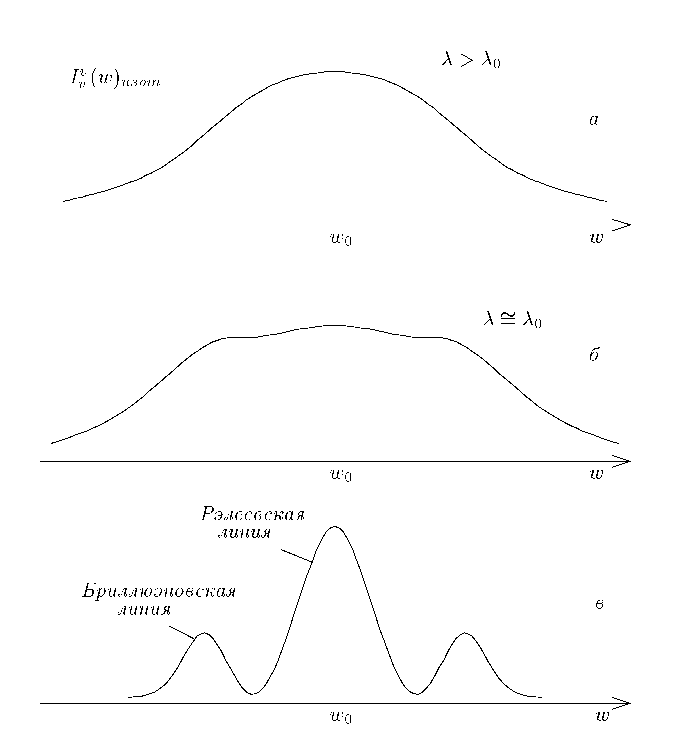
\includegraphics[scale=0.9]{Ris/ris_eps/ris4_4_02.eps}}}

\risp{4.2}{
Схема, показывающая изменения в
спектре изотропного рэлеевского рассеяния}

{\ris при переходе от
разреженного газа ({\it а}) к жидкости ({\it б})}\vskip 2mm\noindent
{\ris $\lambda$ --- средняя длина свободного пробега,
$\lambda_0$ --- длина волны излучения. При переходе к плотному
газу ({\it б}) начинают проявляться бриллюэновские спутники,
обязанные рассеянию на продольных звуковых волнах. В спектре газа
при высоких давлениях, жидкости или твердого тела ({\it
в})($\lambda<\lambda_0$) отчетливо видно наличие боковых
бриллюэновских полос}
\end{figure}


В приведенных уравнениях $P(\vec R,t)$ --- отнесенная к единице объема вероятность
нахождения рассеивателя в точке $\vec R$ в момент времени $t$, а
$I$ --- ток вероятности или поток (число частиц, проходящих через
единичное сечение в единицу времени); $T(\vec R,t)$ ---
температура в точке $\vec R$ в момент времени $t$; ${v}_s$
--- {\it скорость звука} в среде; $C_p$ и $C_v$ --- {\it удельные
теплоемкости} при постоянном давлении и постоянном объеме
соответственно; $\xi$ --- {\it коэффициент телового расширения},
$\eta_s$ и $\eta_B$ - сдвиговая и объемная
вязкости соответственно; $\chi$ --- {\it удельная
теплопроводность};
$\rho$ --- равновесная плотность среды; $\rho={M\over
N_A}\rho_0$, где $M$ --- молекулярный вес, $N_A$ --- число
Авогадро, а $\rho_0$ --- плотность числа частиц.

Применение в гидродинамике приведенных выше линеаризованных
уравнений правомерно при усовии небольших отклонений от
равновесия. Учитывается лишь продольная связь скорости и
плотности. Такое упрощение, когда пренебрегается угловыми
корреляциями между молекулами, ограничивает окончательные
результаты случаем спектров поляризованного излучения. Отметим
также, что плотность, или отнесенная к единице объема верятность,
и температура выбираются в качестве независимых переменных.
Уравнения \eqn{67}, \eqn{68} и \eqn{69} могут быть разрешены
относительно функции $\overline{P}(K,t)$ [фурье-образа функции
$P(\vec R,t)$, как показано в \eqn{64}] путем применения
преобразований Лапласа и Фурье, что дает
$$\overline{P}(K,t)\approx\overline{P}(K,0)\left[\left(1-{C_v\over
C_p}\right)\exp(-\kappa K^2t)+{C_v\over C_p}\exp(-\Gamma
K^2t)\cos{v}_sKt\right],$$
$$\kappa={\chi N_A\over\rho_0C_p},\hskip 4mm
\Gamma={1\over2}\left[{{4\over3}\eta_s+\eta_b\over\rho}+{\chi
N_A\over\rho_0C_v}\left(1-{C_v\over C_p}\right)\right].\noq$$

Здесь $\overline{P}(K,0)$ --- статическая корреляция, которая
будет обсуждаться в настоящем разделе позднее, $\kappa$ ---
{\it коэффициент термодиффузии}, а $\Gamma$ --- {\it эффективный
коэффициент диффузии массы} для звуковых волн в среде. Формула
\eqn{70} справедлива лишь в предельном случае $v_sK\gg\kappa
K^2$.

Первый член в формуле \eqn{70} для $\overline{P}(K,t)$ связан с
флюктуациями энтропии при постоянном давлении. Затухание этих
флюктуаций характеризуется постоянной времени $\tau=1/\kappa\
K^2$. Втоой член в формуле \eqn{70} для $\overline{P}(K,t)$
связан с флюктуациями давления при постоянной энтропии,
приводящими к распространению звуковых вол со скоростью $v_s$.
Этот процесс характеризуется акустической постоянной времени
затухания $\tau_s=1/\Gamma K^2$\  (???) .

Перейдем теперь к рассмотрению спектров рассеянного света.
Подстановка выражения \eqn{70} в \eqn{66} приводит к
корреляционной функции для изотропного рассеяния
$$
C_z(K,t)= AN\alpha^2\overline{P}(K,0)\left(\left(1-{C_v\over
C_p}\right)\exp(-i\omega_0t-\kappa K^2t)+\right. 
$$ $$+ {C_v\over2C_p}\{\exp[-i(\omega_0-v_sK)t-\Gamma K^2t]+ 
$$ $$+ \left.\exp[-i(\omega_0+v_sK)t-\Gamma K^2t]\}\right),
\noq$$
где множитель $\cos v_sKt$ представлен в комплексном виде.
Действительное фурье-преобразование функции $C_z(K,t)$ позволяет
получить изотропный спектр в виде суммы нормированных лоренцевых
функций ${\cal L}_{\kappa}$ и ${\cal L}_{\Gamma}$:
$$
I_{v}^v(K,\omega)_{\rm из}= 
AN\alpha^2\overline{P}(K,0)\left\{\left(1-{C_v\over C_p}\right){\cal
L}_{\kappa}(\omega_0-\omega)+\right. 
$$ $$+ \left.{C_v\over2C_p}\left[{\cal
L}_{\Gamma}(\omega_0-{v}_sK-\omega)+{\cal L}_{\Gamma}
(\omega_0+{v}_sK-\omega)\right]\right\}, 
$$
$$
{\cal L}_{\kappa}(\omega_0-\omega)= {1\over\pi}\left[{\kappa K^2\over(\omega_0-\omega)^2+(\kappa
K^2)^2}\right], 
$$ $${\cal L}_{\Gamma}(\omega_0\pm v_sK-\omega)= {1\over\pi}\left[{\Gamma
K^2\over(\omega_0\pm{v}_sK-\omega)^2+(\Gamma K^2)^2}\right]. 
\noq$$
Изотропный спектр, предсказываемый формулами \eqn{72}, содержит
рэлеевскую линию с центром при частоте
падающего излучения $\omega_0$, имеющую полуширину $\Delta\omega=\kappa K^2$.
Помимо этой центральной линии имеются две линии
Мандельштама-Бриллюэна, сдвинутые по отношению к $\omega_0$ на
$\pm{v}_sK$ в каждую сторону и имеющие полуширины
$\Delta\omega=\Gamma K^2$. Типичные изотропные спектры Рэлея ---
Бриллюэна для $\rm CCl_4$ при трех углах рассеяния приведены на
рис. 4.4.3\  (???) . Экспериментальные значения полуширин и частот
бриллюэновских сдвигов мокут быть использованы для нахождения по
формулам \eqn{72} параметров $\Gamma,\ \kappa$ и $v_s$. Кроме
того, отношение интегральных интенсивностей рэлеевской и
бриллюэновских кривых дает значение $C_p/C_v$ [см. \eqn{72}]:
$$
{I_{\kappa}\over2I_{\Gamma}}= {C_p\over C_v}-1,\hskip 4mm
I_{\kappa}=AN\alpha^2\overline{P}(K,0)\left(1-{C_p\over
C_v}\right)\int\limits_{-\infty}^{\infty}{\cal
L}_{\kappa}(\omega_0-\omega)d\omega, 
$$ $$2I_{\Gamma}= AN\alpha^2\overline{P}(K,0)\left({C_p\over
C_v}\right)\int\limits_{-\infty}^{\infty}{\cal
L}_{\Gamma}(\omega_0+{v}_sK-\omega)d\omega. 
\noq$$

\begin{figure}[tbp]
\centerline{\hbox{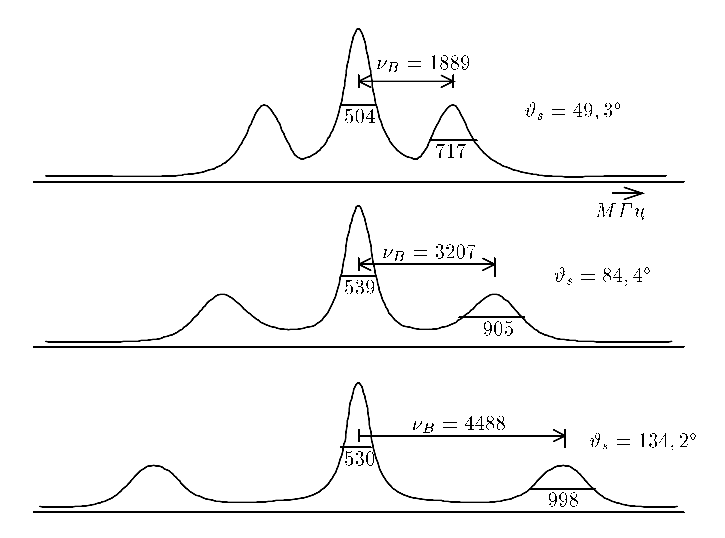
\includegraphics[scale=0.9]{Ris/ris_eps/ris4_4_03.eps}}}

\risp{4.3}{
Спектры изотропного
рассеяния Рэлея-Бриллюэна $I_{v}^v(\omega)^P_{\rm из}$}{\ris для $\rm
CCl_4$ ($T$=293 K) в жидкой фазе для трех различных углов
рассеяния при возбуждении линией $\lambda_0=$6328\angst\ He ---
Ne-лазера.}\vskip 2mm\noindent
{\ris Следует ожидать, что вклад в эти спектры,
обусловленный членом $I_v^v(\nu)^{P}_{\rm аниз}$, будет равным
нулю или очень малым, поскольку величина
($\alpha_{ii}^0-\alpha_{jj}^0$) в случае молекулы $\rm CCl_4$
должна быть равной нулю. Расстояния между центральной частотой и
бриллюэновскими линиями обозначены символом ${\nu_B}$ (все
частоты приведены в мегагерцах). После выделения истинных
спектров из свертки с аппаратной функцией можно найти (путем
подбора) значения параметров $C_p/C_v$, $\Gamma$, $\kappa$ и
$v_s$, при которых эти спектры воспроизводятся согласно формулам
\eqn{72}}
\end{figure}


Этот результат представляет собой хорошо известное отношение
Ландау-Плачека. Из формул \eqn{72} и \eqn{73} очевидно, что при
$C_p=C_v$ интенсивность рэлеевской линии обращается в нуль.

Возвращаясь к обсуждению рис. 4.4.3 для случая $\rm CCl_4$,
отметим, что нанем приведены экспериментальные спектры
$I_v^v(\omega)^P$. Согласно соотношениям \eqn{65},
$$I_{v}^v(\nu)=I_{\rm из}(\nu)+{4\over3}I_{\rm аниз}(\nu).\noq$$
Поскольку интенсивность $I^P_{\rm аниз}(\nu)$ пропорциональна
анизотропии поляризуемости, следует ожидать, что в случае
молекулы $\rm CCl_4$ член $I^P_{\rm аниз}(\nu)$ будет близок к
нулю, что согласуется с данными, приведенными на рис. 4.4.3. Этот член
будет рассмотрен в следующем разделе.

Возвращясь к рис. 4.4.3, отметим, что ширина аппаратной функции
интерферометра Фабри --- Перо, применяемого для регистрации
спектров, больше, чем ширина центральной рэлеевской линии. Это
легко устанавливается, если рассмотреть значение коэффициента
термодиффузии $\kappa$, входящего в формулу \eqn{70}. Значения
удельной теплопроводности при постоянном давлении для $\rm CCl_4$
приведены в табл. 4.4.1. Значение $\kappa$ оказывается равным
$\kappa=N_A\chi/\rho_0C_p=(\chi/\rho C_p)M=7,8\cdot10^{-4}{\rm
см^{2}\cdot с^{-1}}$, где $M$ --- молекулярный вес $\rm CCl_4$.
Отсюда полуширина для наибольшего угла, показанного на рис.
4.4.3 ($134,2^{\circ}$), равна $[K=(2\pi
n/\lambda_0)\sin(\theta_s/2)=2,669\cdot10^5 {\rm см^{-1}}$ для
линии $\lambda_0=6328$\angst\ He --- Ne-лазера]
$\Delta\nu_R=({1\over2}\pi)(\kappa K^2)=8,8$ МГц, что значительно
меньше ширин центральных рэлеевских линий (см. рис. 4.4.3),
наблюдаемых с помощью интерферометра Фабри --- Перо. Таким
образом, согласно рис. 4.4.3 и приведенным вше соображениям,
аппаратная полуширина имеет порядок величины $\Delta\nu=260$ МГц,
и для измерения $\kappa$ необходимо гораздо более высокое
разрешение. Значения $\chi,\ \rho,\ C_p$ и $\kappa$ для некоторых
других веществ приведены в табл. 4.4.2. Все значения $\kappa$
близки к его значениям для $\rm CCl_4$, откуда следует, что
центральные рэлеевские линии являются очень узкими. Как показано
в работе  (???) , авторами которой было определено значение
$\kappa$ для толуола, ширина центральной линии может быть
измерена с помощью оптического смешивания.

Попытаемся теперь на основе формул \eqn{72} дать приближенную
интерпретацию бриллюэновских спектров, изображенных на рисунке
4.4.3. Для этого необходимо, чтобы ширины линий были много
меньше, чем расстояния между центральным рэлеевским спектром и
боковыми бриллюэновскими спектрами. Мы также не будем учитывать
широкие фоновые спектры малой интенсивности, обусловленные
взаимодействием распространяющихся звуковых волн с
внутримолекулярными процессами релаксации. Данные, необходимые
для интерпретации рис. 4.4.3, приведены в табл. 4.4.3.

Прежде всего рассмотрим на основе данных рис. 4.4.3 интегральные
интенсивности. Простое интегрирование кривых и использование
формул \eqn{73} дает отношение Ландау --- Плачека и
результирующее значение $C_p/C_v$ для $\rm CCl_4$, хорошо
согласующиеся с данными табл. 4.4.1.

Значения $K=(2\pi n/\lambda_0)\sin(\theta_s/2)$ для трех углов,
показанных на рис. 4.4.3, при $\lambda_0=6328$\angst\ (He ---
Ne-лазер) и $n=1,459$ (для $\rm CCl_4$) приведены в первом
столбце табл. 4.4.3. Второй столбец содержит значения наблюдаемых
бриллюэновских расщеплений $\nu_B$ согласно данным рис. 4.4.3.
В третьем столбце приведены скорости звука, вычисленные с помощью
вектора рассеяния и значений $\nu_B$, а в четвертом --- длины
волн звуковых колебаний в среде, определяемые формулой
$$\lambda_s={v_s\over\nu_B}={\lambda_0\over2n\sin(\theta_s/2)}={2\pi\over K}.\noq$$

\begin{figure}[tbp]
\centerline{\hbox{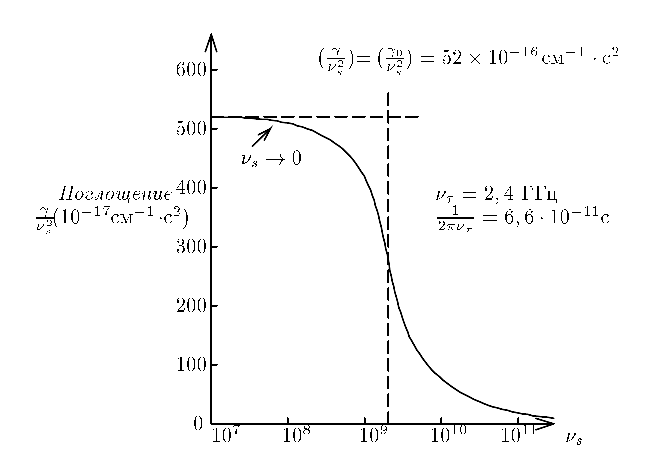
\includegraphics[scale=0.9]{Ris/ris_eps/ris4_4_04.eps}}}

\risp{4.4}{
Результаты измерения
поглощения звука в $\rm CCl_4$ как функция звуковой частоты
$\nu_s$}\vskip 2mm\noindent
{\ris $\gamma({\rm см^{-1}})$ --- коэффициент поглощения; на
графике отложена зависимость ${\gamma\over\nu_s^2}$ от $\nu_s$. В
предельном случае низких частот величину
${\gamma\over\nu_s^2}\rightarrow{\gamma_{0}\over\nu_s^2}$ можно
непосредственно сравнить с величиной $\Gamma_0$, которая, как
видно из формулы \eqn{80}, является предельным низкочастотным
значением коэффициента диффузии массы. Точка перегиба $\nu\tau$
на кривой зависимости ${\gamma\over\nu_s^2}$ от $\nu_s$ ---
частота внутренней релаксации в $\rm CCl_4$
}
\end{figure}


Отсюда видно, что при рассеянии света вперед будут наблюдаться
волны с большой длиной $\lambda_s$, вплоть до $\lambda_s=\infty$,
а при обратном рассеянии --- короткие волны, вплоть до
$\lambda_s=\lambda_0/2n$, где $\lambda_0$ --- длина волны
излучения. Из данных табл. 4.4.3 очевидно также, что скорость
звука зависит от частоты звуковых волн. Низкочастотный предел для
скорости звука $\nu_{s0}$ может быть получен путем
экстраполирования данных табл. 4.4.3 и равен $9,38\cdot10^4{\rm
см\cdot с^{-1}}$ (см. табл. 4.4.1). Изменение скорости звука в
зависимости от частоты. называемое {\it дисперсией} по аналогии с
дисперсией в оптике, весма отчетливо видно на данных табл. 4.4.3.
Развитая здесь упрощенная теория [см. формулы \eqn{72}]

\vbox{{\ris Таблица 4.4.1. Физические параметры соединения
$\rm CCl_4$ при $T=293$ K.}\par\noindent\hangindent 0,7cm\hangafter -5 {\ris Даные взяты из работы
[17][Flygare]. Символом $K^{-1}$ обозначены единицы, обратные
единицам температуры (кельвинам)}
\vskip 2mm
\hskip 0,1cm\hbox{\vbox{\halign{\vrule\hskip 2mm\strut\ris # \hskip 2mm\hfill&
\vrule\hskip 2mm\strut\ris # \hskip 2mm\hfill\vrule\cr
\noalign{\hrule}
Молекулярный вес $M$&153,8 а.е.\cr
Плотность $\rho$&1,595 $\rm г\cdot см^{-3}$\cr
Показатель преломления $n$&1,459\cr
Удельная теплопроводность $\chi$&$2,5\cdot10^{-4}\ {\rm кал\cdot
с^{-1}\cdot см^{-1}\cdot K^{-1}}$\cr
Удельная теплоемкость $C_p$&30,8 $\rm кал\cdot моль^{-1}\cdot
K^{-1}$\cr
$C_p/C_v$&1,47\cr
Скорость звука при низких частотах $v_{s0}$&$9,38\cdot10^4$ $\rm
см\cdot с^{-1}$\cr
Коэффициент диффузии массы при низких$\Gamma_0$&0,11
$\rm см^{2}\cdot с^{-1}$\cr
\hbox{\ \ }частотах $\Gamma_0$&\cr
Коэффициент поглощения звука при низких&$52\cdot10^{-16}{\rm
см^{-1}\cdot с^{2}}$\cr
\hbox{\ \ }частотах, деленный на квадрат звуковой&\cr
\hbox{\ \ }частоты (см. рис. 4.4.4) $\gamma_0/\nu_s^2$&\cr
\noalign{\hrule}}}}}
\vskip 7mm
\vbox{{\ris Таблица 4.4.2. Физические параметры некоторых веществ
при $T=297$ K.}\par\noindent\hangindent 0,7cm\hangafter -5 {\ris
Как следует из формул \eqn{72}, с помощью соотношения
$\Delta\omega=\kappa K^2$ и приведенных в таблице данных можно
вычислить полуширину центральной рэлеевской линии в спектре
изотропного рассеяния. Данные взяты из работы [16][Flygare]. При
использовании приведенных в настоящей таблице единиц имеет место
соотношение $\kappa=\chi/\rho C_p$.}
\vskip 2mm
\hskip 0,1cm\hbox{\vbox{\halign{\vrule\hskip 2mm\strut\ris # \hskip 2mm\hfill&
\vrule\hfill\hskip 2mm\strut\ris # \hskip 2mm\hfill&
\vrule\hfill\hskip 2mm\strut\ris # \hskip 2mm\hfill&
\vrule\hfill\hskip 2mm\strut\ris # \hskip 2mm\hfill&
\vrule\hfill\hskip 2mm\strut\ris # \hskip 2mm\hfill\vrule\cr
\noalign{\hrule}
&&Удельная тепло-&Теплоемкость при&Коэффициент\cr
&$\rho,\ {\rm г\cdot см^{-3}}$&проводность $\chi$,&постоянном
давлении&термодиффузии\cr
&&$10^{-4}\ {\rm кал\cdot см^{-1}\cdot}$&$C_p,\
{\rm кал\cdot г^{-1}\cdot K^{-1}}$&$\kappa,\ 10^{-4}\ {\rm см^{2}\cdot
с^{-1}}$\cr
&&$\rm \cdot с^{-1}\cdot K^{-1}$&&\cr
\noalign{\hrule}
Бензол&0,879&3,3&0,42&8,9\cr
Сероуглерод&1,262&3,8&0,24&12,6\cr
Четыреххлористый&1,595&2,5&0,20&7,8\cr
\hbox{\ \ }углерод&&&&\cr
Уксусная кислота&1,049&4,3&0,48&8,5\cr
Ацетон&0,792&4,2&0,51&10,5\cr
Толуол&0,866&3,5&0,40&9,7\cr
\noalign{\hrule}}}}}

\vskip 7mm
\vbox{\par\noindent\hangindent 0,7cm\hangafter -2{\ris Таблица
4.3.3. Данные, полученные согласно рис. 4.4.3
для изотропного рассеяния Рэлея --- Бриллюэна в $\rm CCl_4$ при
трех значениях угла рассеяния.
}\par\noindent\hangindent 0,7cm\hangafter -5 {\ris
Возбуждение осуществлялось He --- Ne-лазером с длиной волны
излучения в вакууме $\lambda_0=$6328\angst. Числа, стоящие вне
скобок в столбце $\Delta\nu_B$, получени согласно данным рис.
4.4.3. Числа в скобках получены путем оценки полуширин
бриллюэновских линий после исключения из экспериментальных кривых
ирины аппаратной функции (путем выделения истинных
спектров из их свертки с аппаратной функцией).
}
\vskip 2mm
\hskip -1mm\hbox{\vbox{\halign{\offinterlineskip
\vrule\hfill\ris #\strut \hfill&
\vrule\hfill\ris #\strut \hfill&
\vrule\hfill\ris #\strut \hfill&
\vrule\hfill\ris #\strut \hfill&
\vrule\hfill\ris #\strut \hfill&
\vrule\hfill\ris #\strut \hfill&
\vrule\hfill\ris #\strut \hfill&
\vrule\hfill\ris #\strut \hfill&
\vrule\hfill\ris #\strut \hfill&
\vrule\hfill\ris #\strut \hfill\vrule\cr
\noalign{\hrule}
&Вектор&Расстояние&&&Полуши-&Эффективный&Коэффи-&&\cr
&рассеяния&межу
цент-&Скорость&Длина&рина&коэффициент&циент&Время&Длина\cr
Угол&$K=(2\pi n/\lambda_0)\cdot$&ральной
и&звука&волны&бриллю-&диффузии&поглоще-&звуковой&ослабле-\cr
рас-&$\cdot\sin(\theta_s/2)$&бриллю-&
$v_s$=&звука&эновской&массы&ния&релак-&ния\cr
сеяния&($n$=1,459),&эновскими&\hbox{$\mathstrut={2\pi\nu_B\over
K},$}&\hbox{$\lambda_s={v_s\over\nu_B}$},&линии&\hbox{$\mathstrut\Gamma={2\pi\Delta\nu_B\over
K^2},$}&\hbox{$\gamma={\Gamma K^2\over v_s},\mathstrut$}&сации&$1/\gamma,\angst$\cr
&$\ris см^{-1}$&линиями&$\ris см\cdot
с^{-1}$&\angst&$\Delta\nu_B$, МГц&$\ris см^{2}\cdot
с^{-1}$&$\ris см^{-1}$&\hbox{$\mathstrut\tau_s={1\over\Gamma K^2}$}, с&\cr
&&$\nu_B$, МГц&&&&&&&\cr
\noalign{\hrule}
$\,49,3^{\circ}$&$\,1,208\cdot10^5$&$\,1889$&$\,9,8\cdot10^4$&$\,5150$&$\,359(200)$&
$\,8,6\cdot10^{-2}$&$\,1,28\cdot10^4$&$\,7,97\cdot10^{-10}$&$\,7813$\cr
$\,84,4^{\circ}$&$\,1,946\cdot10^5$&$\,3207$&$\,10,4\cdot10^4$&$\,3250$&$\,453(253)$&
$\,4,2\cdot10^{-2}$&$\,1,53\cdot10^4$&$\,6,29\cdot10^{-10}$&$\,6536$\cr
$\,134,2^{\circ}$&$\,2,669\cdot10^5$&$\,4488$&$\,10,5\cdot10^4$&$\,2355$&$\,499(270)$&
$\,2,4\cdot10^{-2}$&$\,1,63\cdot10^4$&$\,5,85\cdot10^{-10}$&$\,6142$\cr
\noalign{\hrule}}}}}
\vskip 5mm

\noindent для интерпретации спектров должна быть модифицирована с учетом
дисперсии. Мы не станем здесь углубляться в детали, а займемся
интерпретацией ширин бриллюэновских линий.

Полуширины бриллюэновских линий приведены в круглых скобках в
шистом столбце табл. 4.4.3. Результирующие значения эффективного
коэффициента диффузии массы приведены в седьмом столбце таблицы;
отметим его сильную зависимость от угла рассеяния или частоты
звука. Низокачастотный предел $\Gamma_0$ можно оценить путем
экстраполяции данных табл. 4.4.3 на случай $\nu_B\rightarrow0$,
откуда $\Gamma_0\approx10,8\cdot10^{-2}{\rm см^{2}\cdot c^{-1}}$.
Это число можно сравнить с низкочастотным предельным значением
коэффициента поглощения $\gamma_0$ для звука с помощью
стандартных методов исследования поглощения звука. В таких
экспериментах получают величину $\gamma/\nu_s^2$ как функцию
$\nu_s$, где $\nu_s$ --- частота звука, а $\gamma$ ---
коэффициент поглощения звука. График завиимости величины
$\gamma/\nu_s^2$ от $\nu_s$ для $\rm CCl_4$ приведен на рис.
4.4.4. Отметим малое изменение ординаты  в области низких частот.
Низкочастотный предел величины $\gamma/\nu_s^2$ в случае $\rm
CCl_4$, определяемый непосредственно с помощью рис. 4.4.4, равен
$$\lim\limits_{\nu_s\rightarrow0}{\gamma\over\nu_s^2}={\gamma_0\over\nu_s^2}=
52\cdot10^{-16}\ {\rm см^{-1}\cdot с^2}.\noq$$
Таким образом, при частотах ниже 300 МГц (см. рис. 4.4.4)
коэффициент поглощения в случае $\rm CCl_4$ равен значенияю
\eqn{76}, умноженному на квадрат частоты звука. низкочастотное
предельное значение величины $\gamma/\nu_s^2$, получаемое в опытах
по поглощению звука, и низкочастотное предельное значение
величины $\Gamma$, получаемое в опытах по рассеянию света,
находятся в очевидной взаимосвязи. Возвращаясь к бриллюэновскому
члену в формулах \eqn{71} или \eqn{72}, отметим, что в предельном
случае низких частот время релаксации звуковой волны равно
$\tau_s=(\Gamma_0K^2)^{-1}$. Таким образом, соответствующий
низкочастотный коэффициент поглощения $\gamma_0$ записывается в
виде
$$\gamma_0={1\over\tau_sv_{s0}}={\Gamma_0K^2\over v_{s0}},\noq$$
где $v_{s0}$ --- предельное значение скорости звука при низких
частотах. Учитывая, что согласно \eqn{75}, $K=2\pi/\lambda_s$,
получаем $\gamma_0=(2\pi)^2\Gamma_0\nu_s^2/v_{s0}^3$. Таким
образом, очевидно, что $Gamma_0$ и $\gamma_0/\nu_s^2$ связаны
соотношением
$${\gamma_0\over\nu_s^2}={(2\pi)^2\Gamma_0\over v_{s0}^3}.\noq$$
Подстановка согласно данным табл. 4.4.1 значений $\Gamma_0$,
$v_{s0}$ и $\gamma_0/\nu_s^2$ для $\rm CCl_4$ показывает, что
соотношение \eqn{78} выполняется. Соотношения \eqn{77} и \eqn{78}
справедливы также при любой частоте, так что можно записать
$${\gamma\over\nu_s^2}={(2\pi)^2\Gamma\over v_s^3},\hskip 4mm
\gamma={1\over\tau_sv_s}={\Gamma K^2\over
v_s}={2\pi\Delta\nu_B\over v_s}.\noq$$
В табл. 4.4.3 приведены также коэффициенты поглощения
(ослабления) $\gamma$, времена релаксации $\tau_s$ и длины
ослабления $1/\gamma$. Последние из полученных соотношений
справедливы для всех частот при сравении опытов по рассеянию света и
по поглощению ультразвука.

Отметим также, что точка перегиба графика зависимости
$\gamma/\nu_s^2$ от $\nu_s$ (рис. 4.4.4) отвечает частоте
внутренней релаксации. При частотах более высоких, чем
$\nu_{\tau}$, ослабление звука значительно меньше, чем при
частотах, лежащих ниже $\nu_{\tau}$. Причин роста поглощения при
низких частотах заключается в том, чтов этом случае может
возбуждасться внутренняя колебательная мода, что приводит к
дополнительному поглощению кинетической энергии
распространяющейся продольной звуковой волны. При частотах,
превышающих $\nu_{\tau}$, попеременные сжатия и расширения
звуковой волны происходят слишком быстро, не позволяя
кинетической энергии поступательного движения превратиться в
потенциальную энергию колебаний молекулы. Напротив, при более
низких частотах звука кинетическая энергия может переодить в
потенциальную и в дальнейшем рассеиваться. В результате точка
перегиба на рис. 4.4.4 соответствует частоте релаксации, а время
релаксации для превращения энергии во внутреннюю равно
$\tau=1/(2\pi\nu_{\tau})$. В случае жидкости $\rm CCl_4$
$\tau=6,6\cdot10^{-11}$ с. Как отмечалось ранее, спектры $\rm
CCl_4$ (рис. 4.4.3) являются суперпозицией изотропных спектров
Рэлея --- Бриллюэна, описываемых формулами \eqn{72}, и широкой
полосы фона, которая обусловлена процессами релаксации,
связанными с переходом кинетической энергии, переносимой
ультразвуком, во внутреннюю энергию колебаний молекул  (???) . (Для
изучения конформационных изменений в молекулах широко применялись
акустические методы исследования, см.  (???) .) Отметим теперь, что
широкая полоса фона обязана процессам колебательной релаксации,
которые наблюдаются с помощью ультразвуковых методов, и
полуширина полосы фона обязана процессам колебательной
релаксации, которые наблюдаются с помощью ультразвуковых методов,
и полуширина полосы фона будет равна величине $\nu_{\tau}$ на
рис. 4.4.4. В случае $\rm CCl_4$ величина $\nu_{\tau}$, как
показывает рис. 4.4.3, имеет порядок бриллюэновских сдвигов, и
для учета этого фона необходимо ввести поправки в спектры Рэлея
--- Бриллюэна. Для многих жидкостей частота внутренней релаксации
меньше, чем обратная величина полуширины центральной рэлеевской
линии, и при интерпретации бриллюэновских спектров не возникает
никаких трудностей.

Ультразвуковые методы широко использовались с целью изучения
процессов релаксации для молекул  (???) . Анализ с этой целью
полуширин бриллюэновских линий стал применяться позднее. В
принципе, согласно рассмотренной здесь простой теории первого
порядка, классические опыты по поглощению звука, в которых
измеряются $\gamma/\nu_s^2$ и $v_s$ как функция $\nu_s$, дают ту
же информацию при использовании формул \eqn{79}, что и
бриллюэновские сдвиги $\nu_B$ и ширины $\Delta\nu_B$,  с помощью
которых находится зависимость скорости и коэффициента диффузии
массы от частоты. В рамках этой теории формулы \eqn{79}
справедливы при любых частотах.

Для получения функции статической корреляции $\overline{P}(K,0)$,
входящей в \eqn{70} и в последующие формулы данного раздела,
вернемся к предыдущему осуждению первых членов в выражениях
\eqn{52} и \eqn{54}, приводящих к изотропному члену в
$I_v^v(\omega)$. Этот член имеет окончательный вид \eqn{71}.
Преобразуя множитель $N\overline{P}(K,0)$ в функции
$C_z(K,t=0)_{\rm из}$, исходя из выражений \eqn{52} и \eqn{54},
получаем
$$
C_z(K,t=0)_{\rm из}= A\alpha^2N\int\exp(i\vec K\cdot\vec R)P(\vec
R,0)dV_s=$$ $$=A\alpha^2N\overline{P}(K,0), 
N\overline{P}(K,0)= N\int\exp(i\vec K\cdot\vec R)P(\vec
R,0)dV_s= 
$$ $$= \left<\sum\limits_{i,j}\exp\{-i\vec K\cdot[\vec r_i(0)-\vec
r_j(0)]\}\right>= 
$$ $$= \left<\sum\limits_{i=j}\exp\{-i\vec K\cdot[\vec r_i(0)-\vec
r_i(0)]\}\right>+ 
$$ $$+ \left<\sum\limits_{i\not=j}\exp\{-i\vec K\cdot[\vec r_j(0)-\vec
r_j(0)]\}\right>, 
\noq$$
где $N=\rho_0V_s$ --- полное число рассеивателей в рассеивающем
объеме $V_s$. Член в скобках переписан в виде суммы собственных
$(i=j)$ и различных членов $(i\not=j)$. Соответственно и функция
$P(\vec R,0)$ может быть представлена как сумма собственной и
различной частей. Собственная часть функции $P(\vec R,0)$
является, очевидно, дельта-функцией от $\vec R$, а второй член
(различный) может быть представлен в виде радиальной функции
праспределения для двух тел $g(\vec R)$[$g(\vec R)$ ---
безразмерная функция]. Таким образом
$$P(\vec R,0)=\delta(\vec R)+\rho_0g(\vec R),\noq$$
где $g(\vec R)$ --- вероятность найти частицу в точке $\vec R$
при условии, что другая частица находится в начале координат.
Функция $g(\vec R)$ на больших расстояниях подчиняется условию
нормировки
$$\lim\limits_{R\rightarrow\infty}g(\vec R)=1.\noq$$
В работе  (???)  приведена типичная парная радиальная функция
распределения, из которой видно, что в случае простых жидкостей
функция $g(\vec R)$ немонотонно изменяется лишь в области, не
превышающей нескольких диаметров молекул. Таким образом, при
больших $\vec R$ функция $P(\vec R,0)$ сводится к усредненной
плотности частиц
$$\lim\limits_{R\rightarrow\infty}P(\vec R,0)=\rho.\noq$$
Подставляя выражение \eqn{81} для $P(\vec R,0)$ в \eqn{80} и
учитывая соотношения
$$\int\exp(i\vec K\cdot\vec R)dV_s=\delta(K)\hskip 4mm и\hskip
4mm\int\exp(i\vec K\cdot\vec R)\delta(\vec R)dV_s=0,$$
можно записать
$$
C_z(K,0)_{\rm
из}= A\alpha^2N\overline{P}(K,0)=A\alpha^2N[S(K)+\rho_0\delta(K)], 
$$ $$S(K)= \int\exp(i\vec K\cdot\vec R)\{\delta(\vec R)+\rho_0[g(\vec
R)-1]\}dV_s. 
\noq$$
Здесь $S(K)$ называют {\it форм-фактором} для жидкости  (???) , а
член, содержащий $\delta(K)$, приводит к рассеянию света вперед,
которой неотличимо от прямого распространения падающего света.
Таким образом, $S(K)$ --- единственный зависящий от $K$ член в
интенсивности рассеянного света, который может быть измерен.
Интеграл в формуле \eqn{84} можно существенно упростить, если
рассматривать излучение в оптическом диапазоне. При этом
расстояния, на которых рассеивается излучение, значительно
больше, чем область от точки $R=0$ до нескольких молекулярных
диаметров, в которой происходят периодические изменения функции
$g(\vec R)$. В подобных условиях можно приближенно положить
$\exp(-i\vec K\cdot\vec R)=1-i\vec K\cdot\vec R+\ldots\approx1,$
откуда получаем
$$\rho_0\int\exp(i\vec K\cdot\vec R)[g(\vec
R)-1]dV_s\approx\rho_0\int[g(\vec R)-1]dV_s.\noq$$
Интеграл в этом окончательном виде может быть вычислен с помощью
методов статистической механики  (???) \ и равен
$$\rho_0\int[g(\vec R)-1]dV_s=\rho_0kT\left(-{1\over V}{\partial
V\over\partial p}\right)_T-1=\rho_0kT\beta_T-1.\noq$$
Здесь $\beta_T=[-(1/V)(\partial V/\partial p)]_T$ ---
изотермическая сжимаемость газа или жидкости при температуре $T$
($\beta_T$ имеет размерность, обратную размерности давления), $k$
--- постоянная Больцмана. Этот окончательный результат не зависит
от $K$. Разумеется, если статические флуктуации охватывают
область до $\lambda_0$ (где $\lambda_0$ --- длина волны
излучения) или используется более коротковолновое излучение, в
подинтегральном выражении в \eqn{85} необходимо учитывать
множитель $\exp(i\vec K\cdot\vec R)$, что приводит к зависимости
окончательного результата от $K$.

Подставляя выражения \eqn{86} и \eqn{85} в \eqn{84}, получаем
значение форм-фактора в предельном случае низких $K$ при
рассеянии излучения оптического диапазона в жидкостях, состоящих
из малых молекул:
$$\lim\limits_{K\rightarrow0}S(K)=kT\rho_0\left(-{1\over
V}{\partial V\over\partial p}\right)_T=kT\rho_0\beta_T.\noq$$

Возвращаясь к выражеию \eqn{84}, отметим, что в предельном случае
низких K, когда величина $1/K$ велика по сравнению со средней
длиной свободного пробега (в газе) или с расстоянием между
рассеивателями (в жидкости), интенсивность изотропно рассеянного
света (при исключении света, рассеянного вперед) пропорциональна
сжимаемости рассеивающей среды
$$\overline{P}(K,0)=\rho_0kT\beta_T.\noq$$
Подстановка этого соотношения в формулы \eqn{71} --- \eqn{73}
приводит к окончательному результату.

В случае идеального газа ($pV=nRT)$ для $n$ молей газа) легко
показать, что $\beta_T=1/p$ и
$\overline{P}(K,0)=kT\rho_0\beta_T=1$. Подставляя этот результат
в \eqn{71} и полагая $t=0$, получаем полные интенсивности от $N$
рассеивателей [приводим также $C_y(K,0)$]
$$
C_z(K,0)= I_v^v=\int\limits_{\infty}^{\infty}I_v^v(\omega)d\omega= 
$$ $$= I_{\rm из}+{3\over4}I_{аниз}={\omega_0^4\over
R^2c^4}I_0N\left[\alpha^2+{4\over45}(\alpha_{aa}-\alpha_{bb})^2\right], 
$$ $$C_y(K,0)= I_h^v=\int\limits_{-\infty}^{\infty}I_h^v(\omega)d\omega=I_{\rm
аниз}=$$ $${\omega_0^4\over
R^2c^4}\left({I_0N\over15}\right)(\alpha_{aa}-\alpha_{bb})^2, 
\noq$$

\vbox{\par\noindent\hangindent 0,7cm\hangafter -2
{\ris Таблица 4.4.4. Изотермические сжимаемости $\beta_T$,
плотности числа частиц $\rho_0$ и множители
$\overline{P}(K,0)=\rho_0kT\beta_T$ для некоторых обычных
жидкостей. Данные взяты из книги [46][Flygare]}\par\noindent\hangindent 0,7cm\hangafter -5 {\ris
Полные интенсивности рассеяния Рэлея --- Бриллюэна
пропорциональны безразмерным множителям $\rho_0kT\beta_T$, где
$k$ --- постоянная Больцмана, $T$ --- температура. Величина
$\rho_0^2kT\beta_T$, умноженная на объем рассеяния $V_s$,
представляет собой полное число молекул, рассеивающих свет.
}
\vskip 2mm
\hskip 0,1cm\hbox{\vbox{\halign{\vrule\hskip 2mm\strut\ris # \hskip 2mm\hfill&
\vrule\hfill\hskip 2mm\strut\ris # \hskip 2mm\hfill&
\vrule\hfill\hskip 2mm\strut\ris # \hskip 2mm\hfill&
\vrule\hfill\hskip 2mm\strut\ris # \hskip 2mm\hfill&
\vrule\hfill\hskip 2mm\strut\ris # \hskip 2mm\hfill&
\vrule\hfill\hskip 2mm\strut\ris # \hskip 2mm\hfill\vrule\cr
\noalign{\hrule}
&&&&$\overline{P}(K,0)=\rho_0kT\beta_T$,&$\rho_0\overline{P}
(K,0)=$\cr
Жидкость&$T,$
K&$\rho_0$,&$\beta_T$,&безразмерная&$=\rho_0^2kT\beta_T$,\cr
&&молекул$\cdot\ris см^{-3}$&$\ris см^{2}\cdot
дин^{-1}$&величина&молекул$\cdot\ris см^{-3}$\cr
\noalign{\hrule}
\vbox to 4mm{\vfil\hbox{\hfil}}
Идеальный&&$2,69\cdot10^{19}$&$9,8\cdot10^{-7}$&$1,0$&$2,69\cdot10^{19}$\cr
\hbox{\ \ }газ ($P=$&&&&&\cr
\hbox{\ \ }$=1$ атм&&&&&\cr
Ацетон&$293$&$1,04\cdot10^{22}$&$12,7\cdot10^{-11}$&$5,34\cdot10^{-2}$&$5,55\cdot10^{20}$\cr
Бензол&$273$&$6,9\cdot10^{21}$&$8,1\cdot10^{-11}$&$2,25\cdot10^{-2}$&$1,55\cdot10^{20}$\cr
$\ris CCl_4$&$293$&$1,04\cdot10^{21}$&$10,7\cdot10^{-11}$&$2,68\cdot10^{-2}$&$0,28\cdot10^{20}$\cr
\noalign{\hrule}}}}}
\noindent где $I_0$ --- интенсивность падающего излчения. На практике
формулы \eqn{89} и рассмотренные ранее формулы \eqn{59} ---
\eqn{63} для степеней деполяризации в газовой фазе широко
используются для определения элементов тензора электрической
поляризуемости молекулы.

В случае плотных газов или жидкостей для оценки интенсивностей
необходимо знать изотермические сжимаемости. Для газов отклонение
от идеальности при высоких давлениях может быть описано
уравнением состояния для плотного газа, таким, например, как
уравнение Ван-вер-Ваалься, или уравнением вириала. С помощью
уравнений состояния могут быть вычислены сжимаемости. В случае
жидкостей изотермические сжимаемости можно легко найти в
литературе. Некоторые типичные значения сжимаемостей для
нескольких обычных жидкостей приведены в табл. 4.4.4.
Изотермическая сжимаемость идеального газа при давлении 1 атм
составляет $\beta_T=1/p=0,98\cdot10^{-6}$ $\rm см^{2}\cdot
дин^{-1}$. В табл. 4.4.4 также приведены плотности числа частиц
$\rho_0$ и безразмерные факторы рассеяния
$\overline{P}(K,0)=\rho_0kT\beta_T$. Последние два столбца
таблицы позволяют дать интерпретацию потери интенсивности
рассеянного света вследствие гасящей интерференции в плотном газе
или жидкости. Данные последнего столбца таблицы, где приведены
значения $\rho_0(\rho_0KT\beta_T)$, можно интерпретировать как
эффективное число молекул, приходящихся на единицу рассеивающего
объема. В случае идеального газа все молекулы в единице объема
рассеивают свет и $\rho_0kT\beta_T=1$. Однако в плотной среде
гасящая интерференция, обусловленная близко расположенными и
коррелированными между собой частицами, уменьшает значение
$\rho_0$ благодаря множителю $\rho_0kT\beta_T$. Из данных
последнего столбца табл. 4.4.4 очевидно также, что для чистых
жидкостей значения полных интенсивностей, приходящиеся на единицу
рссеивающего объема, располагаются в следующем порядке: $I\ ({\rm
ацетон})>I\ ({\rm бензол})>I\ ({\rm CCl_4})$. Аналогичную
информацию об остальных молеулах можно легко получить, используя
известные значения плотностей, изотермических сжимаемостей, а
также соответствующие зависимости этих параметров от давления и
температуры.

Предыдущие результты показывают, что интенсивность рассеянного
света не зависит от $K$, если функция $g(\vec R)$ стремится к 1
на расстояниях, малых по сравнению с $1/K$. Существуют, однако,
определенные условия, когда функция $g(\vec R)$ для излучения
оптического диапазона сильно и немонотонно изменяется на
расстояниях, значительно больших, чем $1/K$. Согласно предыдущему
рассмотрению, наименьшее расстояние, которое может исследоваться
при помощи излучения, рассеянного в обратном направлении
$(\theta=\pi)$, равно $r=\lambda_0/2n$, где $n$ --- показатель
преломления, а $\lambda_0$ --- длина волны излучения. Таким
образом, чтобы можно было наблюдать зависимость от $K$ при
рассеянии излучения оптического диапазона
$(\lambda\approx5000\angst)$ в плотном газе или жидкости,
необходимо наличие пространственных корреляций, действующих на
расстояниях 3000---5000 \angst. Это весьма неправдоподобно для
обычной жидкости, состоящей из малых молекул, и для такой
жидкости не наблюдается какой-либо зависимости полной
интенсивности $I_v^v$ от $K$. Однако вблизи критической точки
имеют место флуктуации, охватывающие большие расстояния, и
независящая от времени пространственная корреляционная функция,
очевидно, принимает вид
$$g(R)-1={A\exp(-R/a)\over R},\noq$$
где $a$ --- длина корреляции двух частиц, а $A$ --- константа.
Результирующий форм-фактор, согласно \eqn{84}, будет иметь ви
$$
S(K)=\int\exp(i\vec K\cdot\vec R )\left[\delta(\vec R)+\rho_0
{A\exp(-R/a)\over R}\right]dV_s= 
$$ $$= 1+{\rho_0A(1/a)\over
K^2+(1/a)^2}, 
\noq$$
и обнаруживается звисимость от $K$ [1, 2][Flygare]. Конечно, в
аморфных телах, полимерах (в твердой фазе) и стеклах могут
существовать статические флуктуации, охватывающие большие
расстояния. Если эти флуктуации или неоднородности коррелируются
на расстояниях порядка $1/K$, то как показано выше, для
интенсивности рассеянного света будет наблюдаться зависимость от
$K$. Рассмотренными методами могут изучаться также статические
неоднородности в двухфазных системах.
\subzag{Анизотропное рэлеевское и комбинационное рассеяние и
изотропное рассеяние в жидкостях; трансляционная и вращательная
диффузия}
Обратимся снова к выражениям \eqn{64} и \eqn{65}. Здесь мы
рассмотрим  функцию $\overline{P}(K,\theta,\varphi,t)$,
определяющую член $I_{\rm аниз}^P(\omega)$, функцию
$\overline{G}(K,\theta,\varphi,t)$, определяющую член $I_{\rm
аниз}^K(\omega)$, и функцию $\overline{G}(K,t)$, определяющую
член $I_{\rm из}^K(\omega)$. На рисунке 4.4.5 приведены спектры
рассеяния нитробензола $I_v^v(\nu)^P=I_{\rm
из}^P(\nu)+{4\over3}I_{\rm аниз}^P(\nu)$ и $I_h^v(\nu)^P=I_{\rm
аниз}^P(\nu)$. Спектр деполяризованного излучения в правой части
рисунка является чисто анизотропным, а кривая слева представляет
собой комбинацию изотропного и анизотропного спектров. Триплет в
спектре $I_{\rm из}^P(\nu)$ обусловлен флуктуациями плотности,
как это было показано в разделе 3.3. Примеры рэлеевских спектров
комбинационного рассеяния для деполяризованного или анизотропного
излучения приведены на рис. 4.4.6. Отметим, что полуширин полос
как $I_{\rm аниз}^K(\nu)$, так и $I_{\rm аниз}^P(\nu)$ в случае
$\rm CS_2$ и бензола значительно больше, чем в случае
нитробензола (рис. 4.4.5). Для рассматриваемых малых молекул
типичные ширины линий при $\theta_s=\pi/2$ (см. рис. 4.4.1)
порядка $0,1\rightarrow10{\rm см^{-1}}$ или
$\Delta\nu=3\cdot10^9\rightarrow3\cdot10^{11}$ Гц.

Прежде всего рассмотрим функцию
$\overline{G}(K,\theta,\varphi,t)$ или $G(\vec
R,\theta,\varphi,t)$ [см. выражение \eqn{64}], определяющую, как
показано, например, на рис. 4.4.6, член $I_{\rm аниз}^K(\nu)$. Мы
помним, что функция $G(\vec R,\theta,\varphi,t)$ состоит
полностью из собственных членов, различные члены равны нулю
вследствие хаотичности фаз колебаний. Таким образом, $G(\vec
R,\theta,\varphi,t)$ содержит лишь одночастичные вклады. Теперь
мы применим гидродинамическую модель Дебая для функции $G(\vec
R,\theta,\varphi,t)$, описывающую как положеие центра масс (ц.
м.) (трансляционная диффузия), так и ориентацию частицы
(вращательная диффузия). В модели Дебая предполагается, что для
переориентации молекулы необходимо множество столкновений.
Используя выражение \eqn{64} для
$\overline{G}(K,\theta,\varphi,t)$, проведем усреднение по
начальным углам, что дает
$$
\overline{G}(K,\theta,\varphi,t)= \int\limits_0^{2\pi}\int\limits_0^{2\pi}
\int\limits_{-1}^1\int\limits_{-1}^1\int\limits_{V_s}\exp(i\vec
K\cdot\vec R)P_2(\cos\theta_0)P_2(\cos\theta)\times 
$$ $$ \times G(\vec R,\theta,\varphi,t)dV_sd\cos\theta_0d\cos\theta
d\varphi_0d\varphi=
$$
$$
= \int\limits_0^{2\pi}\int\limits_{-1}^1\int\limits_{V_s}\exp(i\vec
K\cdot\vec R)P_2(\cos\theta)\zeta(\vec
R,\theta,\varphi,t)dV_sd\cos\theta d\varphi= 
$$ $$= \int\limits_0^{2\pi}\int\limits_{-1}^{1}P_2(\cos\theta)\overline{\zeta}(K,\theta,
\varphi,t)d\cos\theta d\varphi,
\noq$$

\begin{figure}[tbp]
\centerline{\hbox{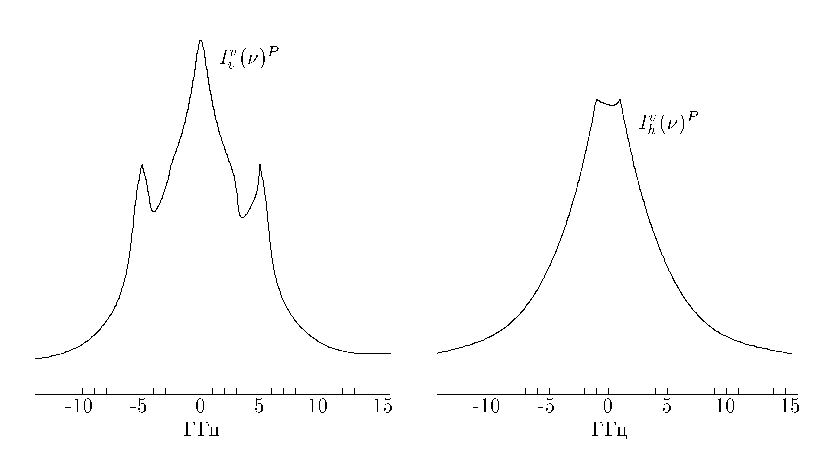
\includegraphics[scale=0.9]{Ris/ris_eps/ris4_4_05.eps}}}

\risp{4.5}{
Спектры $I_v^v(\nu)^P$ и
$I_h^v(\nu)^P\ (\theta_s=\pi/2)$ нитробензола при $T$=297 K
}\vskip 2mm\noindent
{\ris Спектры записаны Барнхэмом и Бертуччи с помощью
интерферометра Фабри-Перо. Возбуждение осуществлялось линией с
$\lambda_0=$5145\angst лазера на ионах $\ris Ar^+$ (см. также
[65][Flygare]). Спектр $I_v^v(\nu)^P$ является комбинацией
изотропной и анизотропной частей $I_v^v(\nu)^P=I^P_{\rm
из}(\nu)+{4\over3}I^P_{\rm аниз}(\nu)$; спектр $I_h^v(\nu)^P$
отвечает лишь анизотропной части $I_h^v(\nu)^P=I^P_{\rm
аниз}(\nu)$}
\end{figure}


\noindent где $\zeta(\vec R,\theta,\varphi,t)$ --- отнесенная к
единице объема вероятность найти в момент времени $t$ ц. м.
молекулы в точке $\vec R$ при ориентации молекулы, определяемой
углами $\theta$ и $\varphi$. Координаты ц. м. и координаты,
определяющие ориентацию, показаны на рис. 4.4.7. Чтобы оценить
функцию $\overline{G}(K,\theta,\varphi,t)$ для отдельной молекулы
в жидкости, применим гидродинамическую модель трансляционной и
вращательной диффузии.

Начнем с рассмотрения одномерной трансляционной диффузии
сферической частицы в случае, когда плотность числа частиц
задается дельта-функцией в плоскости. Исходная дельта-функция,
описывающая концентрацию в плоскости $xy$, схематически
изображена на рис. 4.4.8. Плотность потока $J(y)$ (число частиц,
проходящих через единицу поверхности в единицу времени) из этой
плоскости высокой концентрации пропорциональна градиенту
плотности числа частиц $N(y,t)$ в направлении оси $y$. Константой
пропорциональности является {\it коэффициент диффузии} $D$,
имеющий размерность $\rm см^{2}\cdot с^{-1}$:
$$J(y)=-D{dN(y,t)\over dy}.\noq$$
Можно скомбинировать это уравнение с уравнением непрерывности для
массы вдоль оси $y$ ${dJ(y)\over dy}=-{dN(y,t)\over dt}$, откуда
получается уравнение диффузии
$${dN(y,t)\over dt}=D{d^2N(y,t)\over dy^2}.\noq$$
Применяя для решения этого уравнения пространственное
преобразование Фурье, получаем
$$\int\limits_{\infty}^{\infty}\exp(-iK_yy)\left[{d\over
dt}N(y,t)\right]dy=D\int\limits_{\infty}^{\infty}\exp(-iK_yy)\left[
{d^2N(y,t)\over dy^2}\right]dy,$$

\begin{figure}[tbp]
\centerline{\hbox{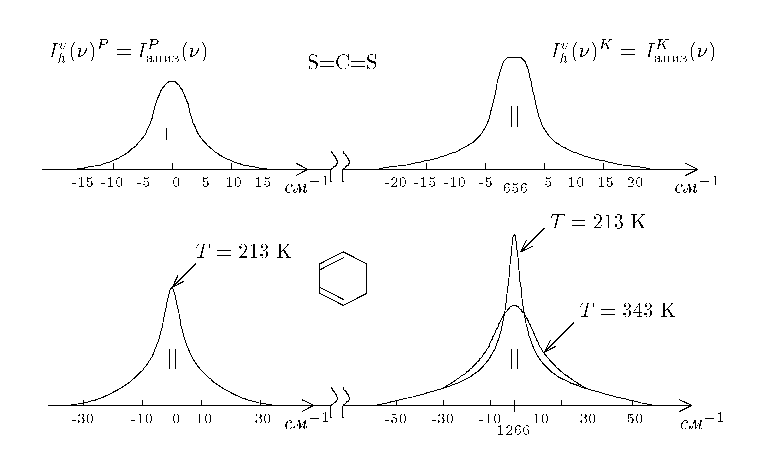
\includegraphics[scale=0.9]{Ris/ris_eps/ris4_4_06.eps}}}

\risp{4.6}{
Спектры
$I_h^v(\nu)=I_{\rm аниз}(\nu)$ рэлеевского (P) и комбинационного
(K)}{\ris рассеяния молекул $\rm CS_2$ и бензола в деполяризованном
свете ($\theta_s=\pi/2$)
}\vskip 2mm\noindent
{\ris Вертикальными шрихами отмечены приближенные ширины
аппаратной функции. Для возбуждения применялось поляризованное
излучение лазера. Спектры рэлеевского рассеяния, показанные на
левой части рисунка, были получены с помощью интерферометра Фабри
--- Перо. Приведенные справа спектры комбинационного рассеяния
записаны с помощью дифракционного оптического спектрографа
(отметим при этом, что 1 $\ris см^{-1}$=30 ГГц). Данные взяты из
работ [66, 67][Flygare], а также из неопубликованной работы
Барнхэма и Бертуччи.
}
\end{figure}


$${d\over dt}\overline{N}(K_y,t)=-K_y^2D\overline{N}(K_y,t).\noq$$
Данное уравнение имеет решение
$$\overline{N}(K_y,t)=\overline{N}(K_y,0)\exp(-K_y^2Dt),\noq$$
где $\overline{N}(K_y,t)$ --- фурье-образ функции $N(y,t)$.
Начальное условие $\overline{N}(K_y,0)$ в пространстве $K_y$
может быть получено из начального условия в обычом пространстве.
Полагая $N(y,0)=\delta(y)$, т. е. дельта-функции для плотности
числа частиц в бесконечной плоскости $xz$ (см. рис. 4.4.8), и
применяя преобразование Фурье, получаем
$$\overline{N}(K_y,0)=\int\limits_{\infty}^{\infty}\exp(-iK_yy)N(y,0)dy=$$
$$=\int\limits_{-\infty}^{\infty}\exp(-iK_yy)\delta(y)dy=1.\noq$$
Подставляя этот результат в выражение \eqn{96}, находим
$$\overline{N}(K_y,t)=\exp(-K_y^2Dt).\noq$$
Теперь можно применить обратное преобразование Фурье для
получения
$$N(y,t)={1\over2\pi}\int\limits_{-\infty}^{\infty}\exp(-K_y^2Dt)\exp(iK_yy)dK_y=$$
$$=\left({1\over4\pi
Dt}\right)^{1/2}\exp\left(-{y^2\over4Dt}\right).\noq$$
Зависимость этой гауссовой функции от времени показана в нижней
части рис. 4.4.8. Можно также записать трехмерное уравнение
диффузии для точечной флюктуации концентрации $N(\vec
R,0)=\delta(\vec R)$ в случае сферических частиц. Оно имеет вид
$${d\over dt}N(\vec R,t)=D\nabla^2N(\vec R,t),\hskip
4mm\overline{N} (K,t)=\exp(- K^2Dt),$$
$$N(R,t)=\left({1\over4\pi
Dt}\right)^{3/2}\exp\left(-{R^2\over4Dt}\right),$$
$$R^2=x^2+y^2+z^2,\hskip 4mm D_x=D_y=D_z=D.\noq$$

Среднеквадратичное расстояние, которое проходит вдоль оси $x$
сферическая диффундирующая частица, первоначально находившаяся в
начале координат ($x=0$), получается путем применения
стандартного статистического усреднения, что дает
$$\overline{(x^2)}=\int\limits_{-\infty}^{\infty}x^2N(x,t)dx=\left(
{1\over4\pi
Dt}\right)^{1/2}\int\limits_{-\infty}^{\infty}x^2\exp\left(
-{x^2\over4Dt}\right)dx=2Dt.\noq$$
Теперь рассмотрим связь коэффициента диффузии $D$ с коэффициентом
трения $f$. Начнем с выражения для случая нейтральной или
заряженной частицы при отсутствии внешнего поля $E_x$:
$$M\ddot x=qE_x-f\dot x.$$
Если сила $qE_x$ равна нулю, частица совершает хаотическое
броуновское движение. Это движение может быть описано путем
замены внешней силы $qE_x$ флюктуационной силой $F(t)$, которая
обусловлена непрерывными столкновениями рассматриваемой частицы с
остальными движущимися частицами среды. Таким образом, имеем
$$F(t)=M\ddot x+f\dot x.\noq$$
Это уравнение Ланжевена, и флуктуационная сила приводит к
броуновскому движению частицы [3, 4][Flygare]. Вычислим теперь
среднюю квадратичную длину пробега вдоль оси $x$, определяемую
хаотической флюктуационной силой \eqn{102}. Для установления
связи между $D$ и $f$ можно будет затем сравнить полученный
результат с выражением \eqn{101}. Значение $\overline{(x^2)}$
можно найти, умножив выражение \eqn{102} для флюктуационной силы
на $x$, что дает $xF(t)=xM\ddot x+xf\dot x.$ Учитывая, что
$d^2x/dt^2=2\dot x^2+2x\ddot x$, получаем
$$xF(t)={M\over2}{d^2\over dt^2}(x^2)-M(\dot
x)^2+{1\over2}f{d\over dt}(x^2),\noq$$
где использовано соотношение $fx\dot x={1\over2}f{d\over dt}x^2$.
Теперь произведем усреднение этого уравнения по большому
промежутку времени, что обозначим скобками. Определив величину
$g=<d/dt(x^2)>$ и замечая, что между $x$ и $F(t)$ нет корреляции
во времени, т. е. $<xF(t)>=0$, находим
$${M\over2}{d\over dt}g=<M(\dot x)^2>-{1\over2}fg.\noq$$
Подстановка значения $<M(\dot x)^2>=kT$ для равномерного
распределения кинетической энергии поступательного движения
приводит к уравнению ($\tau=M/f$)
$${d\over dt}g+{1\over\tau}g={2kT\over M}.\noq$$
Это уравнение имеет решение
$$g(t)=g(t=\infty)\left[1-\exp\left(-{t\over\tau}\right)\right]={2kT\tau\over
M}\left[1-\exp\left(-{t\over\tau}\right)\right].\noq$$
Таким образом, решение в предельном случае больших промежутков
времени, когда выполняется неравенство $t\gg\tau$, имеет вид
$g(\infty)=2kT\tau/M$. Среднее значение $<x^2>$ для промежутков
времени, учитывающих условие $t\gg\tau$, получается в
соответствии с предыдущим определением $g=<dx^2/dt>$ и имеет вид
$$\int\limits_0^1d<x^2>=\int\limits_0^1{2kT\tau\over M}dt.\noq$$
Если при $t=0$ величина $<x^2>=0$, получим
$$\overline{(x^2)}=<x^2>={2kT\tau t\over M}={2kT\over f}t\noq$$
для среднего значения квадрата смещения. Приравнивая соотношения
\eqn{108} и \eqn{101}, выражаем коэффициент диффузии через
константу силы трения
$$D={kT\over f}.\noq$$
Также, отношение подвижности $\mu$ к коэффициенту диффузии $D$
равно
$${\mu\over D}={q\over kT},\noq$$
где $q$ --- заряд иона. Наконец, проводимость $\sigma$ также
связана с коэффициентом диффузии. Согласно полученным результатам
и тому, что $f={q\over\mu}$, имеем
$$\sigma=\rho_0q^2{\tau\over M}={\rho_0q^2\over
f}=\rho_0q\mu={rho_0q^2\over kT}D.\noq$$

Возвращаясь теперь к рассмотрению диффузии, отметим, что формулы
\eqn{93} ---  \eqn{100} принимают иной вид в случае анизотропии
трансляционной диффузии. Подробнее эти вопросы рассмотрены в
 (???) , там же приведены более общие формулы. В случае
аксиально-симметричной молекулы константа $\D_{aa}$
трансляционной диффузии вдоль оси молекулы может отличаться от
констант трансляционной диффузии в перпендикулярном направлении
$\D_{bb}=\D_{cc}$. Вместо уравнения \eqn{93} следует записать
более общее уравнение в неподвижной системе координат
$$J(z)=-\D_{zz}{dN(z,t)\over dz},\noq$$
где $\D_{zz}$ --- коэффициент трансляционной диффузии вдоль оси
$z$ лабораторной системы координат. В отсутствие внешнего или
внутреннего ориентирующего поля жидкость будет изотропной и
$\D_{xx}=\D_{yy}=\D_{zz}$. Однако в случае аксиально-симметричной
молекулы $\D_{aa}\not=\D_{bb}=\D_{cc}$. С использованием
уравнения непрерывности для массы получаем уравнение диффузии
$${dN(z,t)\over dt}=\D_{zz}{d^2\over dz^2}N(z,t).\noq$$
Тензор $\vec{\hbox{\D}}(xyz)$ может быть записан в подвижной системе
координат ($abc$) согласно формулам (С.35). Например,
$\vec{\hbox{\D}}(xyz)=\vec C\vec{\hbox{\D}}(abc)\vec C^*$, где $\vec C$ содержит
направляющие косинусы. На основе соображений, аналогичных
соображениям перед формулами \eqn{35}, находим
$$\D_{zz}=D+{2\over3}(\D_{aa}-\D_{bb})P_2(\cos\theta),$$
где $D=1/3(\D_{aa}+\D_{bb}+\D_{cc})$. Подставляя это выражение в
уравнение \eqn{113}, получаем
$${dN(z,t)\over
dt}=\left[D+{2\over3}(\D_{aa}-\D_{bb})P_2(\cos\theta)\right]{d^2\over
dz^2}N(z,t),\noq$$
где, как и прежде, $\theta$ --- полярный угол в сферической
системе координат. В случае изотропной среды смещения вдоль осей
$x$, $y$ и $z$ эквивалентны, и уравнение \eqn{114} можно
обобщить, что дает
$${dN(\vec R,t)\over
dt}=\left[D+{2\over3}(\D_{aa}-\D_{bb})P_2(\cos\theta')\right]\nabla^2N(\vec
R,t),\noq$$
где $\theta'$ теперь представляет собой угол между осью линейной
молекулы, проходящей через ядра, и вектором $\vec R$. В
отсутствие вращательного движения член с $P_2(\cos\theta')$ в
уравнении \eqn{115} обращается в нуль вследствие изотропного
распределения молекул. Однако, если молекула наряду с
поступательным движением также и вращается, член
$\D_{aa}-\D_{bb}$ приводит к связи поступательного и
вращательного движений. При изотропной диффузии молекул
$\D_{aa}=\D_{bb}=\D_{cc}$ и уравнение \eqn{115} сводится к первой
из формул \eqn{100}.

Используя развитые представления, запишем теперь общее уравнение
для функции $\zeta(\vec R,\theta,\varphi,t)$ входящей в выражение
\eqn{92}. Прежде всего отметим, что оператор Лапласа $\nabla^2$ в
случае аксиально-симметричной молекулы может быть представлен в
виде суммы двух операторов. Первый лапласиан действует на ц. м. и
записывается в декартовой системе координат, а второй действует
на внутренние координаты и записывается в сферической системе
координат
$$
\nabla^2=\nabla^2_{\rm ц.\ м.}+\sum\limits_{i}\left[{1\over
r_i^2}{\partial\over\partial
r_i}\right. \left(r_i^2{\partial\over\partial r_i}\right)+ 
$$ $$ \left.+{1\over r_i^2}{1\over\sin\theta}{\partial\over\partial\theta}\left(\sin
\theta{\partial\over\partial\theta}\right)+{1\over
r_i^2\sin^2\theta}{\partial^2\over\partial\varphi^2}\right], 
$$
$$\nabla^2_{\rm ц.\ м.}={\partial^2\over\partial
X^2}+{\partial^2\over\partial Y^2}+{\partial\over\partial
Z^2},\noq$$
где $r_i$ --- расстояние от ц. м. до $i$-го атома. Подставим
теперь этот лапласиан в уравнение \eqn{115} и применим изложенные
ранее соображения с целью получения уравнения для функции
$\zeta(\vec R,\theta,\varphi,t)$, входящей в \eqn{92}. Отметим
прежде всего, что функция $\zeta(\vec R,\theta,\varphi,t)$ не
зависит от $r_i$. Это позволяет опустить первый член в скобках в
выражении для $\nabla^2$. Опустим также члены $\D_{aa}-\D_{bb}$,
так как в случае почти сферических молекул
$\D_{aa}\approx\D_{bb}$. Отметим, однако, что их влияние можно
учесть с помощью теории возмущений. Окончательно получается
уравнение относительно коэффициента $D$ и коэффициента
вращательной диффузии $\Theta=D\sum\limits_{i}(1/r_i^2)$
(имеющего размерность $\rm с^{-1}$):
$${\partial\zeta(\vec R,\theta,\varphi,t)\over\partial
t}=D\nabla^2_{\rm ц.\ м.}\zeta(\vec R,\theta,\varphi,t)+$$
$$+\Theta\left[{1\over\sin\theta}{\partial\over\partial\theta}\left(
\sin\theta{\partial\over\partial\theta}\right)+{1\over\sin^2\theta}
{\partial^2\over\partial \varphi^2}\right]\zeta(\vec
R,\theta,\varphi,t).\noq$$
Применяя пространственное преобразование Фурье, получаем
$$
{\partial\overline{\zeta}(K,\theta,\varphi,t)\over\partial
t}=\left\{K^2D+\right. 
\Theta\left[{1\over\sin\theta}{\partial\over\partial\theta}\left(
\sin\theta{\partial\over\partial\theta}\right)+\right. 
$$ $$ \left.\left.+{1\over\sin^2\theta} {\partial^2\over\partial
\varphi^2}\right]\right\}\overline{\zeta}(
K,\theta,\varphi,t).
\noq$$
Теперь можно произвести разделение переменных в функции
$$\overline{\zeta}(K,\theta,\varphi,t)=\overline{\zeta}(K,t){\cal
P}(\theta,\varphi),$$
откуда
$${1\over\theta}\left({1\over\zeta}{\partial
\overline{\zeta}\over\partial t}+K^2D\right)={1\over{\cal
P}}\left[{1\over\sin\theta}{\partial\over\partial
\theta}\left(\sin\theta{\partial\over\partial
\theta}\right)+{1\over\sin^2\theta}{\partial^2\over\partial
\varphi^2}\right]{\cal P}.\noq$$
Это равенство соблюдается для всех значений $K,\ \theta$ и
$\varphi$ лишь при условии, что обе его части равны константе.
Обозначая ее $-\lambda$, получаем два дифференциальных уравнения:
$$\left[{1\over\sin\theta}{\partial\over\partial\theta}\left(
\sin\theta{\partial\over\partial\theta}\right)+{1\over\sin^2\theta}
{\partial^2\over\partial \varphi^2}\right]{\cal
P}(\theta,\varphi)=-\lambda{\cal P}(\theta,\varphi),\noq$$
$${\partial\overline{\zeta}(K,t)\over\partial
t}=(-\lambda\Theta-K^2D)\overline{\zeta}(K,t).\noq$$
Если $\lambda=l(l+1)$, уравнение \eqn{120} имеет решение ${\cal
P}(\theta,\varphi)=Y_{lm}(\theta,\varphi)$, где
$Y_{lm}(\theta,\varphi)$ --- сферическая функция. Далее,
уравнение \eqn{121} легко решается и результат имеет вид
$$\overline{\zeta}(K,t)=\overline{\zeta}(K,0)\exp\{-[l(l+1)\Theta+K^2D]t\}.\noq$$
Учитывая, что функция $\zeta(\vec R,t)$ состоит лишь из
собственных членов, можно записать $\zeta(\vec R,0)=\delta(\vec
R)$, откуда $\overline{\zeta}(K,0)=1$. Подставляя этот результат
в выражение \eqn{122}, получаем
$$\overline{\zeta}(K,t)=\exp\{-[l(l+1)\Theta+K^2D]t\}.$$
Наиболее общее решение уравнения \eqn{118} будет линейной
комбинацией полученных частных решений при разных $l$:
$$\overline{\zeta}(K,\theta,\varphi,t)=\sum\limits_{l}A_l
Y_{lm}(\theta,\varphi)\exp\{-[l(l+1)\Theta+K^2D]t\}.\noq$$
Значения коэффициентов $A_l$ можно найти с помощью начальных
условий при $t=0$ для функций \eqn{123} и \eqn{92}. Используя в
формуле \eqn{92} начальное условие $G(\vec
R,\theta,\varphi,0)=\delta(vec
R)\delta(\cos\theta-\cos\theta_0)\delta(\varphi-\varphi_0)$,
получаем
$$
\overline{\zeta}(K,\theta,\varphi,0)= \int\limits_0^{2\pi}\int\limits_{-1}^{1}
P_2(\cos\theta_0)\delta(\cos\theta-\cos\theta_0)\delta(\varphi-\varphi_0)d\cos
\theta_0d\varphi_0= 
$$ $$= P_2(\cos\theta). 
$$
Сравнивая этот результат с начальным условием
$\overline{\zeta}(K,\theta,\varphi,0)=\sum\limits_lA_l
Y_{lm}(\theta_0,\varphi_0)$ при $t=0$ для функции \eqn{123},
находим, что сумма по $l$ должна обрываться на члене с $l=2$ и
что $m=0$ и $A_2=1$. В итоге получаем
$$\overline{\zeta}(K,\theta,\varphi,t)=P_2(\cos\theta)\exp[-(6\Theta+K^2D)t].$$
Подставляя это выражение в \eqn{92} и интегрируя, имеем
$$\overline{G}(K,\theta,\varphi,t)={4\pi\over5}\exp[-(6\Theta+K^2D)t],\noq$$
где $\tau_{\rm ор}=1/6\Theta$ --- время переориентационной
релаксации отдельной частицы. Легко также показать, что в случае
рассматриваемых здесь аксиально-симметричных рассеивателей
функция $\overline{\overline{G}}(K,\theta,\varphi,t)$ [см.
\eqn{64}] равна $1/3$ функции \eqn{124}, т. е.
${1\over3}\overline{G}(K,\theta,\varphi,t)$. Кроме того,
очевидно, что функция $\overline{G}(K,t)$ [см. \eqn{64}] в случае
рассеяния отдельными частицами дается выражением
$$\overline{G}(K,t)=\exp(-K^2Dt).\noq$$
Подставляя эти результаты в соответствующие части корреляционных
функций \eqn{64}, применяя действительное преобразование Фурье и
учитывая формулу \eqn{65}, получаем спектры комбинационного
рассеяния в предельном случае вращательного тушения
$$
I_{\rm из}^K(\omega)= ANf_j{\cal
L}(\omega-\omega_0+\omega_{n'_j,n_j})_{\rm из}, 
$$ $$I_{\rm аниз}^K(\omega)= \left({A\over15}\right)Nh_j{\cal
L}(\omega-\omega_0+\omega_{n'_j,n_j})_{\rm аниз}, 
$$ $${\cal L}(\omega-\omega_0+\omega_{n'_j,n_j})_{\rm из}= 
{1\over\pi}\left\{{DK^2+(1/\tau_j)\over(\omega-\omega_0+\omega_{n'_j,n_j})^2+
[(1/\tau_j)+DK^2]^2}\right\}, 
$$ $${\cal L}(\omega-\omega_0+\omega_{n'_j,n_j})_{\rm аниз}= 
{1\over\pi}\left\{{DK^2+6\Theta+(1/\tau_j)\over
(\omega-\omega_0+\omega_{n'_j,n_j})^2+
[(1/\tau_j)+DK^2+6\Theta]^2}\right\}. 
\noq$$
Обычно из-за вероятностных множителей $N_{n_j},\ f_j$ и $h_j$
[выражения \eqn{64}] в спектрах комбинационного рассеяния
наблюдаются лишь стоксовы переходы [$E_{n_j}<E_{n'_j}$ в формуле
$\omega_{n'_j,n_j}=(E_{n'_j}-E_{n_j})/\hbar$].

Спектр комбинационного рассеяния ${\cal L}(\omega)_{\rm из}$
характеризуется полушириной $\Delta\omega=1/\tau_j+DK^2$, где
$\tau_j$ --- время колебательной релаксации для $j$-го
нормального колебания. Учитывая, что для большинства жидкостей
$D\approx(10^{-4}\ \hbox{---}\ 10^{-5})\ {\rm см^{2}\cdot с^{-1}}$, а
для большинства колебания молекул в жидкостях
$\tau_j\approx10^{-2}$ с, можно с уверенностью положить
$${1\over\tau_j}\gg K^2D\noq$$
для излучения в оптическом диапазоне и любого угла рассеяния.
Таким образом, регистрация спектра комбинационного рассеяния
${\cal L}(\omega)_{\rm из}$ позволяет производить по значениям
полуширин прямое измерение времен колебательной релаксации.
Некоторые значения $\tau_{\rm кол}$, полученные этим способом,
приведены в табл. 4.4.5.

\vskip 3mm
\vbox{\par\noindent\hangindent 0,7cm\hangafter -2{\ris Таблица
4.3.5. Времена колебательной релаксации $\tau_{\rm кол}$ и
времена вращательной релаксации $\tau_{\rm ор}=1/6\Theta$ для
некоторых молекулярных жидкостей, полученные из спектров
комбинационного рассеяния
}
\vskip 2mm

\hskip 0,1cm\hbox{\vbox{\halign{\vrule \strut\hskip 2mm \hfill
\ris#\hfill &\vrule\hskip
2mm\hfill\ris #\hfill\strut
&\vrule\hskip 2mm\hfill\ris #\hfill\strut&\vrule\hskip
2mm\hfill\ris #\hfill\strut\vrule\cr
\noalign{\hrule}
& Колебатель-
& &\cr
Молекула & ный переход, & \vbox{\vskip 1mm\hbox{$\tau_{\rm
кол},\ 10^{-12}$ с\ }}&
\vbox{\vskip 1mm\hbox{$1/6\Theta=\tau_{\rm
ор}$,\ }}\cr
&$\rm см^{-1}$&&$10^{-12}$ с\ \cr
\noalign{\hrule}
\hbox{\vbox to 4mm{}}$\rm CS_2$ & 656 & $10,6\ ^{1)}$ & $1,5\ ^{1)}$\cr
Ацетонитрил & 2943 & $3,2\ ^{2)}$ & $0,9\ ^{2)}$\cr
Метилиодид & 525 & $2,0\ ^{1)}$ & $1,5\ ^{1)}$\cr
& 1245 & $2,0\ ^{1)}$ & $1,4\ ^{1)}$\cr
Хлороформ & 667 & $2,0\ ^{1)}$ & $1,5\ ^{1)}$\cr
& 3019 & $1,1\ ^{1)}$ & $1,5\ ^{1)}$\cr
Бромоформ & 222 & $4,1\ ^{1)}$ & $5,3\ ^{1)}$\cr
& 3019 & $1,2\ ^{3)}$ & $4,4\ ^{3)}$\cr
Бензол & 992 & $4,7\ ^{4)}$ & $2,8\ ^{4)}$\cr
Гексафторбензол & 558 & $2,2\ ^{1)}$ & $6,6\ ^{1)}$\cr
\noalign{\hrule}}}}}
\vskip 1mm
{\ris $^{1)}$ См.  (???) .\hskip 2mm $^{2)}$ См.  (???) .\hskip 2mm
$^{3)}$ См.  (???) .\hskip 2mm$^{4)}$ См.  (???) .}
\vskip 2mm

Спектр комбинационного рассеяния ${\cal L}(\omega)_{\rm аниз}$
имеет полуширину, равную $\Delta\omega=1/\tau_j+DK^2+6\Theta$.
Типичные значения $\Theta$ в случае малых молекул лежат в
интервале $10^9\ \hbox{---}\ 10^{12}\ {\rm с^{-1}}$. Если
применяется излучение в оптическом диапазоне, можно с
уверенностью положить
$$6\Theta\gg DK^2\noq$$
для любого угла рассеяния. Таким образом, регистрация спектра
комбинационного рассеяния ${\cal L}(\omega)_{\rm аниз}$ позволяет
по полуширине и известному значению $\tau_j$ производить прямое
измерение коэффициента вращательной диффузии $\Theta$ или времени
ориентационной релаксации $\tau_{\rm ор}=1/6\Theta$. Некоторые
значения $\tau_{\rm ор}$, полученные таким методом, приведены в
табл. 4.4.5. Разумеется, на опыте регистрируются спектры
$I_v^v(\nu)^K=I_{\rm из}^K(\nu)+{4\over3}I_{\rm аниз}^K(\nu)$ и
$I_h^v(\nu)^K=I_{\rm аниз}^K(\nu)$. Спектр $I_{\rm из}^K$ может
быть выделен из спектра $I_v^v(\nu)^K$ путем вычитания
${4\over3}I_h^v(\nu)^K$.

Помня о нашей исходной модели аксиально-симметричной почти
сферической молекулы, могущей изменять направление своей оси
симметрии, отметим, что величины $\Theta$ и $D$ могут быть
выражены через динамическую вязкость $\eta$ и радиус частицы $r$,
согласно [ (???) ,  (???) ,  (???) ], следующим образом:
$$D={kT\over f}={kT\over6\pi\eta r},\hskip 4mm
\Theta={kT\over8\pi\eta r^3}={kT\over6V^*\eta},\noq$$
где $k$ --- постоянная Больцмана, $r$ --- радиус сферической
молекулы, $V^*={4\over3}\pi r^3$ --- эффективный объем молекулы.

Рассмотрим теперь спектр $\overline{P}(K,\theta,\varphi,t)$
[см. \eqn{64}]. Функция $\overline{P}(K,\theta,\varphi,t)$
схожа с рассмотренной выше функцией
$\overline{G}(K,\theta,\varphi,t)$, которая содержит лишь
собственные член, однако функция $\overline{P}(K,\theta,\varphi,t)$
содержит как собственные, так и различные члены. Следует ожидать,
таким образом, что в разнице между $\overline{P}(K,\theta,\varphi,t)$
и $\overline{G}(K,\theta,\varphi,t)$ [или между $I_{\rm
аниз}^P(\nu)$ и $I_{\rm аниз}^K(\nu)$ соответственно] выявится
влияние различны членов или двухчастичных ориентационных парных
корреляций. Прямое сравнение спектров $I_{\rm аниз}^P(\nu)$ и
$I_{\rm аниз}^K(\nu)$ для $\rm CS_2$ и бензола приведено на рис.
4.4.6. Тщательный анализ данных показывает, что в случае молекул
$\rm CS_2$ полуширина спектра $I_{\rm аниз}^P(\nu)$ несколько
меньше, чем спектра $I_{\rm аниз}^K(\nu)$. Этот факт отражает
влияние парных ориентационных корреляций. Однако в случае бензола
рассматриваемые ширины одинаковы, что указывает на отсутствие
влияния ориентационных парных корреляций.
\vskip 3mm
\vbox{\par\noindent\hangindent 0,7cm\hangafter -2{\ris Таблица
4.3.6. Времена вращательной переориентации $\tau_{\rm ор}^P$,
полученные с помощью полуширин деполяризованных рэлеевских линий
$\Delta\omega=1/\tau_{\rm ор}^P$ (см., например, рис. 4.4.6)
}\par\noindent\hangindent 0,7cm\hangafter -5 {\ris
Темпеатура равна примерно 300 K
}
\vskip 2mm

\hskip 0,1cm\hbox{\vbox{\halign{\vrule \strut\hskip 2mm
\hfill\ris #\hfill &\vrule\hskip
2mm\hfill\ris #\hfill\strut\vrule
&$\,$\vrule\hskip 2mm\hfill\ris #\hfill\strut&\vrule\hskip
2mm\hfill\ris #\hfill\strut\vrule\cr
\noalign{\hrule} {Молекула}& \vbox{\vskip 1mm\hbox{$\tau_{\rm
ор}^{\bar P}\cdot10^{-12}$ с\ }}
& Молекула &\vbox{\vskip 1mm\hbox{$\tau_{\rm
ор}^{\bar P}\cdot10^{-12}$ с}}\cr \noalign{\hrule}
${\rm CS_2}$& $1,8\ ^{1)}$ &\hbox{\vbox to 4mm{}} Бромоформ & $10,1\ ^{3)}$ \cr
Ацетонитрил & $1,7\ ^{1)}$ & Бензол & $2,9\ ^{4)}$ \cr
Метилиодид & $2,3\ ^{1)}$ & Гексафторбензол & $14,0\ ^{5)}$ \cr
Хлороформ & $2,9\ ^{2)}$ &&\cr\noalign{\hrule}}}}}
\vskip 1mm
{\ris $^{1)}$ См.  (???) .\hskip 2mm $^{2)}$ См.  (???) .\hskip 2mm
$^{3)}$ См.  (???) .\hskip 2mm$^{4)}$ См.  (???) .\hskip 2mm$^{5)}$
См.  (???) .}
\vskip 2mm

\noindent Значения $\tau_{\rm
ор}^P=1/\Delta\omega$ [где $\Delta\omega$ --- полуширина спектра
$I_{\rm аниз}^P(\nu)$] для некоторых молекул приведены в табл.
4.3.6. Сравнение $\tau_{\rm ор}^P$, согласно табл. 4.4.6, со
значениями $\tau_{\rm ор}$, согласно табл. 4.4.5, показывает, что
$\tau_{\rm ор}\leq\tau_{\rm ор}^P$, т. е. что влияние
ориентационных парных корреляций приводит к существенно большим
временам вращательной релаксации. Парные ориентационные
корреляции оказывают также влияние и на интегральные
интенсивности анизотропного рэлеевского и комбинационного
спектров. Согласно выражениям \eqn{64}, \eqn{65}, предыдущему
обсуждению и соображениям, аналогичным приведенным перед
формулами \eqn{80}, находим
$$I_{\rm аниз}^{P}=\int\limits_{\infty}^{\infty}I_{\rm
аниз}^{P}(\omega)d\omega=\left({AN\over3}\right){(\alpha_{aa}-\alpha_{bb})^2\over4\pi}\overline{P}
(K,\theta,\varphi,0),\noq$$
$$I_{\rm аниз}^{K}=\int\limits_{\infty}^{\infty}I_{\rm
аниз}^{K}(\omega)d\omega=\left({AN\over3}\right){h_j\over4\pi}\overline{G}
(K,\theta,\varphi,0),\noq$$
$$
N \overline{P}(K,\theta,\varphi,0)=N\overline{G}(K,\theta,\varphi,0)+ 
$$ $$ +\left<\sum\limits_{i\not=j}P_2(\cos\theta)_{0i}P_2(\cos\theta)_{0j}\exp
\{-i\vec K\cdot[\vec r_i(0)-\vec r_j(0)]\}\right>, 
\noq$$
где $I_{\rm аниз}^K$ относится к $j$-му нормальному колебанию,
$N=V_s\rho_0$ --- число рассеивателей. Подставляя выражение
\eqn{124} и предполагая, что вращательное и поступательное
движения разделяются, получаем
$$N\overline{P}
(K,\theta,\varphi,0)={4\pi\over5}N+
\left<\sum\limits_{i\not=j}P_2(\cos\theta)_{0i}
P_2(\cos\theta)_j\right>.\noq$$
Остающееся независимое суммирование по $i$ и $j$ ($i\not=j$)
проводится по всем парам молекул, находящимся в элементе объема $V_s$.
Таким образом, если все молекулы идентичны, все члены в одной из
сумм будут одинаковы, так что можно записать
$$N\overline{P}(K,\theta,\varphi,0)=
{4\pi\over5}N+(N-1)\left<\sum\limits_{j}P_2
(\cos\theta)_iP_2(\cos\theta)_j\right>,\noq$$
где последний член включает усреднение по большому промежутку
времени $(N-1)$ одинаковых $i$-ых членов, просуммированных по $j$
($i\not=j$). Применяя теперь формулу сложения сферических функций и
выражая произведение $P_2(\cos\theta)_iP_2(\cos\theta)_j$ через
полиномы $P_2(\cos\theta_{ij})$, где $\theta_{ij}$ --- угол между
осями аксиальной симметрии для пары молекул $ij$, и заменяя
усреднение по времени усреднением по пространству (на основании
эргодической гипотезы), получим
$$N\overline{P}(K,\theta,\varphi,0)=
{4\pi\over5}N+{4\pi\over5}(N-1)\left<\sum\limits_{i}P_2
(\cos\theta_{ij})\right>={4\pi\over5}Ng_2,\noq$$
$$g_2=1+{N-1\over
N}\left<\sum\limits_{j}P_2(\cos\theta_{ij})\right>\approx
1+\left<\sum\limits_{j}P_2(\cos\theta_{ij})\right>,\noq$$
где на последнем этапе принято $(N-1)/N=1$, что справедливо при
большом числе частиц в рассеивающем объеме. Здесь $g_2$
--- {\it фактор ориентационных парных корреляций}.
Член $<\sum_{j}P_2(\cos\theta_{ij})>$ представляет
собой сумму средних значений
$P_2(\cos\theta_{ij})={1\over2}(3\cos^2\theta_{ij}-1)$ для
$(N-1)$
пары молекул $ij$ в жидкости. Подставляя результат \eqn{133} в
выражение для $I_{\rm аниз}^P$ в формулах \eqn{130}, а функцию
\eqn{124} в выражение для $I_{\rm аниз}^K$ в формулах \eqn{130},
получаем интегральные интенсивности
$$I_{\rm
аниз}^{P}={1\over15}Ag_2N(\alpha_{aa}-\alpha_{bb})^2,\hskip 4mm
I_{\rm аниз}^K={A\over15}Nh_j.\noq$$

\begin{figure}[tbp]
\centerline{\hbox{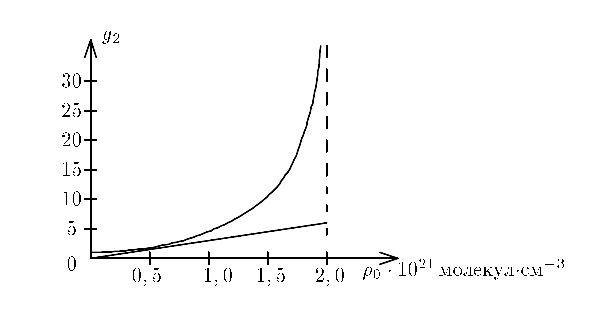
\includegraphics[scale=0.9]{Ris/ris_eps/ris4_4_07.eps}}}

\risp{4.7}{
Экспериментальное определение величины $g_2$ как функции
плотности $\rho_0$ на основе}\centerline{\ris соотношения
$I^P=\int\limits_{-\infty}^{\infty}I_{\rm аниз}^{P}(\nu)d\nu$
[см. формулу \eqn{134}]
}\par\noindent
{\ris Исследовалась система, представляющая собой изотропную
жидкость {\it n}-метоксибензилиден-{\it н}-бутиланилин
(МББА), при температуре 318 К, которая превышает температуру
перехода для жидкокристаллической фазы. Данные взяты из работы
???}
\end{figure}

Таким образом, из полученных результатов вытекает, что
если в чистом растворе некоррелирующих мономерных
аксиально-симметричных молекул произойдет внезапная димеризация,
сопровождающаяся выстраиванием осей симметрии, и если корреляции
между различными димерами будут отсутствовать, то
$<\sum\limits_{j}P_2(\cos\theta_{ij})>=1$ и $g_2=2$,
что приведет к возрастанию интенсивности спектра.
Если же при димеризации оси симметрии окажутся взаимно
перпендикулярными, то
$<\sum\limits_{j}P_2(\cos\theta_{ij})>=-{1\over2}$,
$g_2={1\over2}$, и интенсивность спектра $I_{\rm аниз}^P$
уменьшится. На рис. 4.4.9 показана диаграмма зависимости $g_2$ от
плотности (полученная с использованием спектра $I_{\rm аниз}^P$)
в случае изотропной жидкости МББА, стержнеобразные молекулы
которой образуют жидкий кристалл с выстраиванием стержней.
Полученное на основе измерения спектра $I_{\rm аниз}^P$ и
результирующих значений $g_2$, доказательство выстраивания осей с
ростом плотности является вполне убедительным. Разумеется,
$g_2\rightarrow N$ при приближении системы к жидкокристаллической
фазе.

Для предельного случая диффузии Дебая, когда для переориентации
молекул необходимо большое число столкновений, Кейс и Кивелсон
 (???)  показали, что зависящая от времени часть корреляционной
функции также содержит $g_2$ [см. выражение \eqn{124} при
$\tau_{\rm ор}=1/6\Theta$]:
$$\overline{P}(K,\theta,\varphi,t)={4\pi\over5}g_2\exp\left[-\left(
{1\over\tau_{\rm ор}g_2}+K^2D\right)t\right],\noq$$
где значения $\tau_{\rm ор}g_2=\tau_{\rm ор}^P$, полученные с
помощью полуширины спектра $I_{\rm аниз}^P(\omega)$, приведены в
табл. 4.4.6.
\numq 0
\def\eqnpf#1{(II.#1)}
\def\noqpf{\global\advance\numq by 1\eqno(\hbox{II.\the\numq})}
\vfil
\eject
\noindent{\glv Приложение II}
\vskip 3mm
\noindent{\prgf Некоторые сведения из математики}
\vskip 2mm
\noindent{\bf Матрицы}
\vskip 2mm
Квадратный или прямоугольный массив некоторых чисел называют {\it
матрицей}
$${\bf A}=\left(\matrix{{\rm A}_{11}&{\rm A}_{12}&{\rm
A}_{13}&\ldots\cr
{\rm A}_{21}&{\rm A}_{22}&{\rm A}_{23}&\cr
{\rm A}_{31}&{\rm A}_{32}&{\rm A}_{33}&\cr
\vdots&&&\ddots\cr
}\right).\noqpf$$

Суммой двух матриц {\bf A} и {\bf B} является новая матрица {\bf
C}, каждый элемент которой представляет собой сумму
соответствующих элементов {\bf A} и {\bf B}, а именно:
$${\bf A}+{\bf B}={\bf C},$$
$$\left(\matrix{{\rm A}_{11}&{\rm A}_{12}&{\rm
A}_{13}&\ldots\cr
{\rm A}_{21}&{\rm A}_{22}&{\rm A}_{23}&\cr
{\rm A}_{31}&{\rm A}_{32}&{\rm A}_{33}&\cr
\vdots&&&\ddots\cr
}\right)+\left(\matrix{{\rm B}_{11}&{\rm B}_{12}&{\rm
B}_{13}&\ldots\cr
{\rm B}_{21}&{\rm B}_{22}&{\rm B}_{23}&\cr
{\rm B}_{31}&{\rm B}_{32}&{\rm B}_{33}&\cr
\vdots&&&\ddots\cr
}\right)=\left(\matrix{{\rm C}_{11}&{\rm C}_{12}&{\rm
C}_{13}&\ldots\cr
{\rm C}_{21}&{\rm C}_{22}&{\rm C}_{23}&\cr
{\rm C}_{31}&{\rm C}_{32}&{\rm C}_{33}&\cr
\vdots&&&\ddots\cr
}\right),$$
$${\bf C}=\left(\matrix{{\rm A}_{11}+{\rm B}_{11}&{\rm
A}_{12}+{\rm B}_{12}&{\rm
A}_{13}+{\rm B}_{13}&\ldots\cr
{\rm A}_{21}+{\rm B}_{21}&{\rm A}_{22}+{\rm B}_{22}&{\rm
A}_{23}+{\rm B}_{23}&\cr
{\rm A}_{31}+{\rm B}_{31}&{\rm A}_{32}+{\rm B}_{32}&{\rm
A}_{33}+{\rm B}_{33}&\cr
\vdots&&&\ddots\cr
}\right).\noqpf$$
Очевидно, что отдельные элементы матриц связаны между собой
соотношениями
$${\rm C}_{ij}={\rm A}_{ij}+{\rm B}_{ij}.\noqpf$$
Матрицы {\bf A}, {\bf B} и {\bf C} не обязательно квадратные, но
у них должно быть одинаковое число строк и одинаковое число
столбцов. Умножение матрицы на некоторую постоянную величину
$\varepsilon$ сводится к умножению каждого элемента этой матрицы
на данную постоянную:
$$\varepsilon{\bf A}=\left(\matrix{
\varepsilon{\rm A}_{11}&\varepsilon{\rm A}_{12}&\ldots\cr
\varepsilon{\rm A}_{21}&\varepsilon{\rm A}_{22}&\cr
\vdots&&\ddots\cr
}\right).\noqpf$$
Также непосредственно вводится правило умножения матриц:
$$\left(\matrix{{\rm A}_{11}&{\rm A}_{12}&{\rm
A}_{13}&\ldots\cr
{\rm A}_{21}&{\rm A}_{22}&{\rm A}_{23}&\cr
{\rm A}_{31}&{\rm A}_{32}&{\rm A}_{33}&\cr
\vdots&&&\ddots\cr
}\right)\left(\matrix{{\rm B}_{11}&{\rm B}_{12}&{\rm
B}_{13}&\ldots\cr
{\rm B}_{21}&{\rm B}_{22}&{\rm B}_{23}&\cr
{\rm B}_{31}&{\rm B}_{32}&{\rm B}_{33}&\cr
\vdots&&&\ddots\cr
}\right)=\left(\matrix{{\rm C}_{11}&{\rm C}_{12}&{\rm
C}_{13}&\ldots\cr
{\rm C}_{21}&{\rm C}_{22}&{\rm C}_{23}&\cr
{\rm C}_{31}&{\rm C}_{32}&{\rm C}_{33}&\cr
\vdots&&&\ddots\cr
}\right).\noqpf$$
Каждый элемент матрицы {\bf C} получается соответствующим
перемножением строки матрицы {\bf A} на столбец матрицы {\bf B}
(число столбцов в матрице {\bf A} при этом должно равняться числу
строк в матрице {\bf B}):
$${\rm C}_{ij}=\sum\limits_{k}{\rm A}_{ik}{\rm B}_{ki}.\noqpf$$
{\it Комплексно-сопряженная} матрица (обозначаемая звездочкой)
получается, если все элементы исходной матрицы заменить на
комплексно-сопряженные [с заменой $i=(-1)^{1\over2}$ на $-i$ во
всех элементах матрицы]:
$${\bf A}^*=\left(\matrix{
{\rm A}_{11}^*&{\rm A}_{12}^*&\ldots\cr
{\rm A}_{21}^*&{\rm A}_{22}^*&\cr
\vdots&&\ddots\cr
}\right).\noqpf$$
{\it Транспонирование} матрицы (обозначается тильдой, $\widetilde{\bf
A}$) сводится к замене строк на столбцы и обратно в исходной
матрице:
$$\widetilde{\bf A}=\left(\matrix{{\rm A}_{11}&{\rm A}_{21}&{\rm
A}_{31}&\ldots\cr
{\rm A}_{12}&{\rm A}_{22}&{\rm A}_{33}&\cr
{\rm A}_{31}&{\rm A}_{23}&{\rm A}_{33}&\cr
\vdots&&&\ddots\cr
}\right).\noqpf$$
Матрица, {\it эрмитово-сопряженная} данной (обозначается крестом,
${\bf A}^{\dagger}$), получается как транспонированная
комплексно-сопряженная
$${\bf A}^{\dagger}=\widetilde{\bf A^*}=
\left(\matrix{{\rm A}^*_{11}&{\rm A}^*_{21}&{\rm
A}^*_{31}&\ldots\cr
{\rm A}^*_{12}&{\rm A}^*_{22}&{\rm A}^*_{33}&\cr
{\rm A}^*_{31}&{\rm A}^*_{23}&{\rm A}^*_{33}&\cr
\vdots&&&\ddots\cr
}\right).\noqpf$$
Легко убедиться, что транспонированное произведение матриц равно
произведению соответствующих транспонированных матриц, взятому в
обратном порядке
$$
{\bf C}={\bf AB},\hskip 4mm {\bf C}^*={\bf A^*B^*},
\widetilde{\bf C}=\widetilde{\bf B}\widetilde{\bf A},\hskip 4mm {\bf
C}^{\dagger}={\bf B}^{\dagger}{\bf A}^{\dagger}.
\noqpf$$
Исходя из этих простых примеров, можно построить и более сложные
произведения матриц.

Квадратную матрицу ${\bf u}$ называют {\it унитарной}, если она
удовлетворяет условию
$${\bf uu}^{\dagger}={\bf u}^{\dagger}{\bf u}={\bf 1}=
\left(\matrix{
1&0&0&\ldots\cr
0&1&0&\cr
0&0&1&\cr
\vdots&&&\ddots\cr
}\right).\noqpf$$
Матрица {\bf 1} --- единичная. Представляя элементы матрицы
\eqnpf{11} в явном виде, получаем
$$\sum\limits_{j}u^{\dagger}_{kj}u_{jl}=\sum\limits_{j}u^*_{jk}u_{jl}=\delta_{kl},\noqpf$$
где $\delta_{kl}$ --- дельта-символ Кронекера, равный
$$\delta_{kl}=\left\{\matrix{1,\ \hbox{если}\ k=l,\cr
0,\ \hbox{если}\ k\not=l.\cr}\right.\noqpf$$
Очевидно, что
$${\bf 1A=A,\hskip 4mm B1=B},\noqpf$$
где порядок квадратной единичной матрицы {\bf 1}  должен
равняться числу столбцов матрицы {\bf A} и числу строк матрицы
{\bf B}.

Матрица ${\bf B}^{-1}$, обратная квадратной матрице {\bf B},
определяется следующим образом:
$${\bf BB}^{-1}={\bf B}^{-1}{\bf B}={\bf 1}.\noqpf$$
Отсюда следует, что детерминант матрицы {\bf B} должен быть
отличен от нуля. В случае унитарной матрицы, для которой ${\bf
u^{\dagger}u=1}$,
$${\bf u}^{\dagger}{\bf u}={\bf u}^{-1}.\noqpf$$
В частном случае, когда все элементы унитарной матрицы {\bf u}
действительны
$${\bf u}^{\dagger}{\bf u=1}=\widetilde{\bf u}{\bf u};\hskip
4mm\widetilde{\bf u}={\bf u}^{-1}.\noqpf$$
Таким образом, транспонирование действительной унитарной матрицы
эквивалентно ее обращению.

Другим типом произведения матриц является {\it прямое
произведение} ${\bf A}\times{\bf B}$, которое образуется
умножением всех элементов матрицы {\bf A} на все элементы матрицы
{\bf B}:
$${\bf A}\times{\bf B}=\left(\matrix{
{\rm A_{11}}&{\rm A_{12}}\cr
{\rm A_{21}}&{\rm A_{22}}\cr
}\right)\times\left(\matrix{
{\rm B_{11}}&{\rm B_{12}}\cr
{\rm B_{21}}&{\rm B_{22}}\cr
}\right)=$$
$$=\left(\matrix{
{\rm A_{11}B_{11}}&{\rm A_{11}B_{12}}&{\rm A_{12}B_{11}}&{\rm
A_{12}B_{12}}\cr
{\rm A_{11}B_{21}}&{\rm A_{11}B_{22}}&{\rm A_{12}B_{21}}&{\rm
A_{12}B_{22}}\cr
{\rm A_{21}B_{11}}&{\rm A_{21}B_{12}}&{\rm A_{22}B_{11}}&{\rm
A_{22}B_{12}}\cr
{\rm A_{21}B_{21}}&{\rm A_{21}B_{22}}&{\rm A_{22}B_{21}}&{\rm
A_{22}B_{22}}\cr
}\right).\noqpf$$
\vskip 3mm
\noindent
{\bf Векторы и их связь с матрицами}
\vskip 2mm
{\it Скаляр} --- это обычное число. {\it Вектор} --- число, в
котором содержится также информация о направлении в пространстве.
Векторы и скаляры подчиняются обычным ассоциативному и
дистрибутивному законам умножения.

Вектор в трехмерном пространстве задется составляющими по трем
осям декартовой системы координат согласно формуле
$${\bf A}={\bf \hat i}A_x+{\bf\hat j}A_y+{\bf\hat k}A_z,\noqpf$$
где ${\bf\hat i},\ {\bf\hat j}$ и ${\bf\hat k}$ --- единичные
векторы, направленные по осям $x,\ y$ и $z$ соответственно, а
$A_x,\ A_y$ и $A_z$ --- величины составляющих вектора по
соответствующим осям декартовой системы координат. Можно записать
выражение \eqnpf{19} и иначе, в виде произведения матрицы-строки
и матрицы-столбца:
$${\bf A}=({\bf\hat i}{\bf\hat j}{\bf\hat k})\left(\matrix{A_x\cr
A_y\cr A_z\cr}\right)={\bf\hat i}A_x+{\bf\hat j}A_y+{\bf\hat
k}A_z.\noqpf$$

В результате скалярное произведение двух векторов {\bf A} и {\bf
B} в декартовых координатах имеет вид
$${\bf A\cdot B}=(A_x A_y A_z)\left(\matrix{{\bf\hat
i}\cr{\bf\hat j}\cr{\bf\hat k}\cr}\right)\cdot({\bf\hat i}{\bf\hat j}{\bf\hat k})
\left(\matrix{B_x\cr B_y\cr B_z\cr}\right)$$

